\section{L'assioma della scelta}
L'assioma della scelta è stato introdotto da \href{https://en.wikipedia.org/wiki/Ernst_Zermelo}{\textcolor{purple}{Ernst Zermelo}} nel 1904, per dimostrare che ogni insieme è ben ordinabile.
Si potrebbe dubitare del valore di una dimostrazione ottenuta introducendo un assioma ad hoc, è tuttavia opportuno osservare che l'assioma della scelta è stato usato prima di Zermelo, ma senza accorgersene.
Quindi Zermelo non ha tanto costruito un nuovo principio, quanto piuttosto riconosciuto la necessità di codificare un principio già applicato, ma in modo impreciso.
Inoltre, gli assiomi che abbiamo introdotto fin'ora non permettono, per esempio, né di affermare né di negare la buona ordinabilità di $\RR$. Quindi, se si vuole dare una risposta al problema dell'esistenza di un buon ordine 
di $\RR$, che sia positiva o negativa, questa deve per forza venire da un nuovo assioma. In questo senso, Zermelo dice che il teorema del buon ordinamento è ragionevole perché segue da una ipotesi - l'assioma della scelta - ragionevole.
Anzi, così ragionevole che i matematici l'hanno usato senza neppure accorgersi che questo assioma è effettivamente un'ipotesi.

\begin{axiom}[Assioma della scelta (AC)]
	\label{ax9}
	Dato un insieme $X$ di insiemi non vuoti, esiste una \vocab{funzione di scelta} $f : X \rightarrow \bigcup X$ tale che $\forall a \in X \; f(a) \in a$\footnote{Cioè la funzione manda ogni elemento $a$ di $X$ in un suo elemento.}.
	In simboli:
	\[ \forall X (\emptyset \not \in X) \rightarrow (\exists f \in {}^X\left(\bigcup X\right) \; \forall a \in X \; f(a) \in a)\footnote{Letteralmente le funzioni di scelta ``scelgono'' un elemento in cui mandare tutto l'insieme, preso a sua volta come elemento.}
		\]
\end{axiom}

L'assioma della scelta è, di frequente, applicato per \vocab{fissare infiniti elementi}. Per esempio, dovendo costruire una successione $x_n$ che tende a $+\infty$, capita di ragionare dicendo
\textcolor{MidnightBlue}{per ogni $n \in \NN$ fisso $x_n > n$ che abbia questa o quella proprietà che mi interessano.}\\
Formalmente, in questo ragionamento, stiamo dicendo \textcolor{MidnightBlue}{considero}:
\[ X = \{ \rbrack n,+\infty\rbrack | n \in \NN\}
	\]
\textcolor{MidnightBlue}{e considero} $f : X \rightarrow \bigcup X \subseteq \RR$ \textcolor{MidnightBlue}{una funzione di scelta per $X$. Ora pongo $x_n = f(]n,+\infty])$}. Si pone quindi una domanda: perché non ci serve alcun assioma per fissare un elemento - come a dire \textcolor{MidnightBlue}{considero un
numero $\varepsilon$ tale che etc.} - ma ci serve per fissarne infiniti?\\

Il principio che, sapendo che ci sono oggetti che godono di una certa proprietà, ci permette di fissarne uno, è una legge logica.\\
Questa legge, da un lato, è valida in ogni \vocab{teoria del primo ordine}, non solo nella teoria degli insiemi. D'altro canto, può essere vista come una mera scorciatoia nei ragionamenti, perché se da $\exists x \; \varphi(x)$ possiamo dedurre una $\psi$ che non menziona $x$,
fissando un $x$ che soddisfa $\varphi(x)$, allora si può dimostrare che, a patto di presentare il ragionamento nella maniera opportuna, la conclusione $\psi$ può essere raggiunta senza bisogno di fissare $x$\footnote{Cioè se fissando $x$ il predicato diventa una proposizione vera, con cui continuare il ragionamento, si dimostra che si può arrivare a $\psi$ anche senza 
bisogno di fissare $x$, in questo senso è come se l'azione di ``fissare'' un elemento fosse un'azione vuota, nel senso che il ragionamento formalmente può essere portato avanti anche senza richiederla, ma noi lo facciamo perché ci è comodo ragionare così, ma si può equivalentemente procedere senza effettivamente farlo.}. In questo senso, la possibilità
di fissare un oggetto - cioè dare un nome ad un oggetto - è una legge del pensiero: una caratteristica del modo in cui ragioniamo.\\
Tecnicamente, questa legge è vendicata [nel senso di rivendicata] dal \vocab{teorema di completezza di Gödel}, che dice che la logica del primo ordine è quella giusta per catturare una nozione molto naturale di \vocab{modello}.\\
L'assioma della scelta, d'altra parte, \textcolor{red}{si può vedere} come un modo per fissare elementi, ma \textcolor{red}{si concretizza} in un enunciato insiemistico, che asserisce l'esistenza di un certo insieme: la funzione di scelta.
Non si tratta dunque di una caratteristica del nostro modo di ragionare - di una legge del pensiero - perché nulla ci obbliga a pensare in termini insiemistici, e, d'altro canto, nulla obbliga gli insiemi a fare quello che il nostro intuito ci dice dovrebbero fare.
Insomma, questo è l'intoppo: che non sappiamo esprimere il concetto di \textcolor{MidnightBlue}{fissare infinite variabili} se non tramite l'espediente di \textcolor{MidnightBlue}{fissare una singola funzione di scelta}\footnote{Che fissi in un solo colpo tutti gli infiniti elementi.}. Tuttavia, per fare questo dobbiamo asserire l'esistenza di un certo insieme, appunto la funzione di scelta,
che, si può dimostrare, non segue dagli assiomi 1-8. Bando alle ciance.

\begin{note}[Ogni funzione surgettiva ha inversa destra]
	AC equivale all'affermazione che ogni funzione surgettiva ha un inversa destra, ossia:
	\[ \forall f : X \rightarrow Y \; \text{surgettiva}\;\exists g : Y \rightarrow X \; f \circ g = \id_Y
		\]
\end{note}

\begin{proof}
	Verifichiamo che l'enunciato sopra è un fatto equivalente ad AC.
	\begin{itemize}
		\item[$\boxed{\Longrightarrow}$] Consideriamo l'insieme delle controimmagini via $f$ degli elementi di $Y$:
		\[ Z \Mydef \{A \in \ps(X) | \exists y \in Y \; \overbrace{\forall x \in X \; x \in A \leftrightarrow f(x) = y}^{A = f^{-1}(y)}\}
			\]
		Per la surgettività di $f$ gli elementi di $Z$ sono tutti non vuoti, dunque per \hyperref[ax9]{AC} esiste $h : Z \rightarrow \bigcup Z = X$ funzione di scelta.
		Definiamo quindi $g(y) \Mydef h(f^{-1}(y))$ - più precisamente $g(y) = h(\{x \in X | f(x)  = y\})$, segue che:
		\[ f \circ g(y) = f(g(y)) = f(h(\{x \in X | f(x)  = y\}))
			\]
		ed essendo $h$ una funzione di scelta, si ha che $h(A) \in A$, dunque $h(f^{-1}(y)) \in f^{-1}(y)$, quindi fa un certo elemento nella controimmagine di $y$, fissato dalla nostra funzione di scelta $h$, e, indipendentemente da quale sia, torniamo indietro con $f$, dunque:
		\[ f(z) = y \qquad \text{con $z \in f^{-1}(y)$}
			\]
		\item[$\boxed{\Longleftarrow}$] Verifichiamo ora che da questo fatto derivi l'assioma della scelta. Sia $X$ un insieme di insiemi non vuoti, consideriamo l'insieme $X' = \{(a,A) \in \left(\bigcup X\right) \times X | a \in A \land A \in X\}$.
		La funzione:
		\[ f : X' \rightarrow X : (a,A) \mapsto A
			\]
		è banalmente surgettiva, quindi per ipotesi ha un'inversa destra $g : X \hookrightarrow X'$ che manda $A$ in una coppia $(a,A)$ per qualche $a \in A$\footnote{Che fissa $a \in A$ senza scriverlo esplicitamente.}.
		Ora quindi la funzione:
		\[ h : X \rightarrow \bigcup X : A \mapsto \text{prima componente di $g(A)$}
			\]
		è una funzione di scelta per $X$, perché prendiamo la prima componente di $g(A)$, che sta in $A$, e questa è determinata da $g$, cioè $h(A) \in A$.
	\end{itemize}
\end{proof}

L'assioma della scelta forma, insieme ai due enunciati seguenti - il teorema del buon ordinamento ed il lemma di Zorn - una terna classica di proposizioni equivale, nel senso che gli assiomi 1-8, unitamente ad una qualunque delle tre proposizioni, implicano le altre due.

\begin{theorem}[Teorema del buon ordinamento - o di Zermelo]
	\label{buon_ordinamento}
	Ogni insieme è ben ordinabile, ovvero:
	\[ \forall S \; \exists < \in S \times S \; (S,<)\;\text{è un buon ordinamento}
		\]
\end{theorem}

\begin{definition}[Sottocatena - maggiorante - massimale]
	Dato $(S,<)$ un ordine parziale abbiamo che:
	\begin{itemize}
		\item una \vocab{sottocatena} è un $A \subseteq S$ tale che $(A,<_{|A})$, cioè $A$ con la restrizione dell'ordine di $S$ ad $A$, è un ordine totale
		\item un \vocab{maggiorante} di $A \subseteq S$ è un $x \in S$ tale che $\forall y \in A \; y \leq x$
		\item $x \in S$ è un elemento \vocab{massimale} se $\neg \exists y \in S \; x < y$.
	\end{itemize}
\end{definition}

\begin{lemma}[Lemma di Zorn]
	\label{Zorn}
	Ogni insieme parzialmente ordinato, in cui ogni sottocatena ammette un maggiorante ha elementi massimali.
\end{lemma}

\begin{theorem}[AC $\iff$ buon ordinamento $\iff$ Zorn]
	Le tre affermazioni \hyperref[ax9]{assioma della scelta}, \hyperref[buon_ordinamento]{teorema del buon ordinamento} e \hyperref[Zorn]{lemma di Zorn} sono equivalenti -
	ossia si implicano vicendevolmente assumendo gli assiomi 1-8.
\end{theorem}

\subsection{\texorpdfstring{Buon ordinamento $\rightarrow$ AC}{Buon ordinamento implica AC}}

\begin{proof}
	(Buon ordinamento $\rightarrow$ AC)\\
	Dato $S$ insieme di insiemi non vuoti, fissiamo, per il \hyperref[buon_ordinamento]{teorema del buon ordinamento}, un buon ordine $\prec$ su $\bigcup S$. Allora la funzione:
	\[ f : S \rightarrow \bigcup S : x \mapsto \min_{\prec}(x)
		\]
	è una funzione di scelta per $S$ [perché naturalmente $\min_\prec (x) \in x$, e il fatto che per Zermelo sappiamo che $\prec$ è un buon ordinamento su $S$, ma non sappiamo esplicitamente cosa faccia, ci dice che, tale funzione fissa il minimo, ma non sappiamo necessariamente chi sia, perché non 
	conosciamo esplicitamente $\prec$, da cui la funzione di scelta].
\end{proof}

\subsection{\texorpdfstring{AC $\rightarrow$ buon ordinamento (idea)}{AC implica buon ordinamento (idea)}}
\textcolor{MidnightBlue}{Dimostreremo questo risultato tramite la catena di deduzioni AC $\rightarrow$ Zorn $\rightarrow$ buon ordinamento. Tuttavia conviene studiare l'idea di una dimostrazione diretta.}

\begin{proof}
	(AC $\rightarrow$ buon ordinamento (idea))\\
	Fissiamo un insieme $X$, per \hyperref[ax9]{AC}, esiste una funzione di scelta:
	\[ f : \ps(X) \setminus\{\emptyset\} \rightarrow \bigcup \ps(X) = X : A \mapsto f(A) \in A
		\]
	Ora vorremmo mettere in ordine gli elementi di $X$ come segue;
	\[ F(0) = x_0 = f(X) \qquad F(1) = x_1 = f(X \setminus \{x_0\}) \qquad F(2) = x_2 = f(X \setminus \{x_0,x_1\}) \qquad\ldots
		\]
	ogni volta scegliendo un elemento nuovo fra quelli che rimangono ancora da elencare. Chiaramente non è detto che questo procedimento termini
	in una quantità numerabile di passi, per cui potremmo dover definire $x_\omega = f(X\setminus\{x_0,x_1,x_2,\ldots\})$ e, più in generale, possiamo definire per ricorsione transfinita:
	\[ F(\alpha) = f(X \setminus\{x_\beta | \beta < \alpha\}) = f(X \setminus F[\alpha])
		\]
	Questa cosa non può funzionare per tutti gli ordinali, cioè $F$ non è ben definita, perché da un certo punto in poi $F[\alpha] = X$ e non possiamo usare la funzione di scelta sul vuoto, se per assurdo $F[\alpha] \subsetneq X$ per ogni $\alpha \in \Ord$, allora staremmo immergendo la classe degli ordinali in un insieme, tramite $\alpha \mapsto F(\alpha) \in X$,
	che è ancora assurdo (si avrebbe che l'Hartogs $H(X)$ si immerge in $X$ ad un certo punto o anche è violato Burali-Forti).\\
	Per rimediare a questo inconveniente definiamo quindi
	\[ F(\alpha) = \begin{cases}
		f(X \setminus F[\alpha]) &\text{se $F[\alpha] \subsetneq X$} \\
		\spadesuit &\text{altrimenti}
	\end{cases}
		\] 
	che ora è una funzione classe $\Ord \to X \cup \{\spadesuit\}$ ben definita. A questo punto consideriamo $\beta := \min\{\gamma : F(\gamma) = \spadesuit\}$, che è ben definito poiché è un insieme di ordinali, non vuoto in 
	quanto se fosse vuoto ricadremmo in uno dei due assurdi citati sopra, pertanto si ha che $F[\beta] = X$ e $F_{|\beta}$ è una mappa iniettiva in quanto $f$ è iniettiva per definizione, per cui $X$ è in bigezione con l'ordinale $\beta$
	e quindi può essere ben ordinato mediante un ordinamento indotto, per cui abbiamo ottenuto Zermelo.
\end{proof}

\subsection{\texorpdfstring{Zorn $\rightarrow$ buon ordinamento}{Zorn implica buon ordinamento}}

\begin{proof}
	(Zorn $\rightarrow$ buon ordinamento)\\
	Vogliamo dimostrare che un insieme $S$ è ben ordinabile. Consideriamo:
	\[ \begin{split}
		T &:= \{f : \alpha \to S | \;\text{$\alpha < H(S)$ e $f$ iniettiva}\} \textcolor{MidnightBlue}{=\{\text{funzioni iniettive da un ordinale a $S$}\}} \\
		  &= \{f \in \ps(H(S) \times S) | \; \text{$f$ è una funzione iniettiva e $\Dom(f) \in \Ord$}\}
	\end{split}
		\]
	\footnote{Deve essere necessariamente che $\alpha < H(S)$, perché se $\alpha \geq H(S)$ si immergesse in $S$, allora una restrizione dell'immersione permetterebbe di immergere anche $H(S)$ in $S$, che è assurdo, dunque 
	gli ordinali che si possono immergere in $S$ sono soltanto quelli più piccoli del suo Hartogs. Si noti inoltre che $T$ è non vuoto perché c'è sempre la funzione da 0 a $S$ o da 1 ad $S$, se $S$ è non vuoto.}Osserviamo
	che $T$ è parzialmente ordinato dalla relazione d'ordine $f < g \equiv f \subseteq g$. Diamo per buono che $(T,<)$ soddisfa le ipotesi del 
	lemma di Zorn, e quindi esiste $f \in T$ massimale rispetto alla relazione $<$. Abbiamo che $f$ è surgettiva, infatti, se non lo fosse $S \setminus \Imm(f) \ne \emptyset$, dunque esiste $y \in S \setminus \Imm(f)$ e possiamo definire:
	\[ f' = f \cup \{(\Dom(f),y)\}
		\]
	dove $\Dom(f)$ è l'ordinale successore al massimo del dominio di $f$, ed $f'$ è iniettiva perché unione di funzione iniettive su insiemi in arrivo disgiunti, quindi avremmo $f' > f$ e $f \in T$, che va contro la massimalità di $f$, quindi è assurdo.
	Abbiamo quindi che $S$ è in bigezione con $\Dom(f) \in \Ord$, dunque è bene ordinabile, perché possiamo indurre un buon ordinamento su $S$ via $f$, e quindi abbiamo il teorema del buon ordinamento.\\
	\textcolor{purple}{Verifica delle ipotesi del del lemma di Zorn}\\
	Dobbiamo verificare che data $P \subseteq T$ una sottocatena di $T$, ha sempre un maggiorante, verifichiamo che $f := \bigcup P$ è il maggiorante in questione. In primis osserviamo che $f$ è una funzione ben definita, infatti, essendo un'unione di funzioni
	ci basta verificare, per un'osservazione vista in precedenza, che per ogni $g_1,g_2 \in P$ se $x \in \Dom(g_1) \cap \Dom(g_2)$, allora $g_1(x) = g_2(x)$ (in tal modo $f$ è effettivamente una funzione), essendo che $(P,<_{|P})$ è totalmente ordinato, allora vale WLOG $g_1 > g_2$,
	ovvero $g_2 \subseteq g_1$, dunque le due funzioni coincidono su $x$, perché una estende l'altra.\\
	Verifichiamo ora che $f$ è iniettiva, se $f(x) = f(y)$, allora esistono, per definizione di unione, $g_1,g_2 \in P$ tali che $g_1(x) = f(x)$ e $g_2(y) = f(y)$, ma, come prima, essendo $P$ totalmente ordinato, vale WLOG $g_1 \supseteq g_2$, per cui $g_1(x) = g_2(y) = g_1(y)$, ed essendo $g_1 \in T$ è iniettiva, dunque si conclude $x = y$.
	Osserviamo inoltre che, per le proprietà degli ordinali:
	\[ \Dom(f) = \bigcup\{\Dom(g) | g \in P\} = \sup\{\Dom(g) | g \in P\}
		\]
	dove il sup è un ordinale per quanto visto sugli insiemi di ordinali. A questo punto $f$ è ben definita, ha dominio un ordinale ed è iniettiva, per cui $f \in T$. Ci resta da verificare che $f$ sia un maggiorante per $P$, ma ciò è banale per come abbiamo costruito $f$, infatti:
	\[ \forall g \in P \; g \subseteq \bigcup P = f \equiv g \leq f
		\]
\end{proof}
 
\subsection{\texorpdfstring{AC $\rightarrow$ Zorn}{AC implica Zorn}}

\begin{proof}
	(AC $\rightarrow$ Zorn)\\
	Sia $(S,<)$ un insieme parzialmente ordinato. Supponiamo che ogni sottocatena di $S$ abbia un maggiorante e che, per assurdo, $S$ non abbia elementi massimali.
	Questa assunzione si traduce nel fatto che ogni elemento di $S$ ammette un maggiorante stretto in $S$, $\forall x \in S \; \exists y \in S \; y > x$ (è la negazione della definizione di esistenza di un elemento massimale), ora per ipotesi ogni sottocatena $A$ ammette un maggiorante in $S$, che può essere a sua volta maggiorato strettamente per quanto appena detto,
	dunque ogni sottocatena ammette un maggiorante stretto - d'altronde se ci fosse una sottocatena con un maggiorante non stretto, che quindi non può essere maggiorato strettamente da nessun altro elemento di $S$, allora sarebbe un elemento massimale per quest'ultimo, contraddicendo la nostra ipotesi.\\
	Sia $f : \ps(S) \setminus \{\emptyset\} \to \bigcup \ps(S) \setminus \{\emptyset\} = S$ una funzione di scelta per i sottoinsiemi di $S$. L'idea è ora di costruire per induzione transfinita una funzione classe crescente [quindi iniettiva] $F : \Ord \to S$ - che chiaramente non può esistere 
	perché altrimenti $F_{|H(S)}$ sarebbe un'immersione di $H(S)$ in $S$, e dunque avremmo l'assurdo (alternativamente anche perché violeremmo Burali-Forti). Vorremmo costruire $F$ tramite la ricorsione transfinita forte come segue:
	\[ F(\alpha) = f(\{\text{maggioranti stretti di $F[\alpha]$}\})
		\]
	perché questa costruzione abbia senso, è necessario che $F_{|\alpha}$ sia [debolmente] crescente, un questo modo $F[\alpha]$ è una sottocatena di $S$ e, per l'osservazione sopra, l'insieme dei maggioranti stretti non è vuoto, ed ha senso applicare ad esso la funzione di scelta $f$, e dunque la $F$ è ben definita,
	inoltre è strettamente crescente per costruzione.\\
	Per assurdo consideriamo il minimo (possiamo farlo per l'ipotesi assurda e per i soliti motivi sugli insiemi di ordinali) $\alpha$ tale che $F_{|\alpha}$ non è [debolmente] crescente. Quindi esistono $\gamma < \delta < \alpha$ tali che $F(\gamma) \not \leq F(\delta)$ ($S$ non è detto sia un ordine totale,
	quindi non possiamo dire che $F(\gamma) > F(\delta)$). Però siccome $\delta < \alpha$, per la minimalità di quest'ultimo, $F_{|\delta}$ è crescente, per cui $F(\delta)$ è ben definita
	ed è un maggiorante stretto di $F[\delta]$, quindi, in particolare, $F(\gamma) < F(\delta) \; \lightning$.\\
	\textcolor{red}{\underline{Questo modo di procedere, però, contiene un'imprecisione formale}}\\
	Per applicare il teorema di ricorsione transfinita alla costruzione di $F$ dobbiamo scrivere $F(\alpha) = G(F_{|\alpha})$. La $G$ della costruzione precedente è:
	\[ G(h) = f(\{\text{maggioranti stretti dell'immagine di $h$}\})
		\]
	Questa però non è una funzione classe definita da $V$ a $V$ (in arrivo può essere qualsiasi cosa), come richiesto dal teorema di ricorsione transfinita, perché non è definita se l'immagine di $h$ non ha maggioranti stretti in $S$. Il ragionamento si aggiusta così: si fissa $\spadesuit \not \in S$ e si definisce:
	\[ F(\alpha) = \begin{cases}
		f(\{\text{maggioranti stretti di $F[\alpha]$}\}) &\text{se $F_{|\alpha} : \alpha \to S$ è crescente} \\
		\spadesuit &\text{altrimenti}
	\end{cases}
		\] 
	ora tutti i casi sono coperti ed è lecito applicare il teorema di ricorsione transfinita. Se $F$ non fosse una funziona classe crescente $\Ord \to S$, ci sarebbe il minimo $\alpha$ tale che $F_{|\alpha}$ non è
	$\alpha \to S$ crescente, e, ragionando come prima si ottiene un assurdo.\\
	Ricapitolando, negando la tesi, abbiamo costruito una funzione classe crescente, dunque iniettiva $\Ord \to S$, che non può esistere per il teorema di Hartogs.
\end{proof}

\begin{remark}
	Il problema sottile che si presenta sopra è che nell'enunciato del teorema di ricorsione transfinita la $G$ richiesta deve essere ben definita su tutto $V$, e, prima della correzione (in particolare abbiamo dovuto aggiungere un valore per l'immagine 
	per tutti gli insiemi che non sono ordinali) nel caso sopra, non lo era.
\end{remark}

\pagebreak
\subsection{Conseguenze immediate di AC}

\begin{proposition}[Tutti le cardinalità infinite sono aleph]
	Ogni insieme è equipotente ad un ordinale iniziale\footnote{Per gli insiemi finiti lo sapevamo già, senza bisogno di AC.}. In particolare, ogni cardinalità infinita è un aleph.
\end{proposition}

\begin{proof}
	Per il \hyperref[buon_ordinamento]{teorema del buon ordinamento} ogni insieme è bene ordinabile, quindi isomorfo ad un ordinale, e per le proprietà
	degli ordinali iniziali (cioè sono i rappresentati di tutte le cardinalità \textcolor{purple}{di ordinali}), ogni insieme è equipotente ad un ordinale iniziale.
	La seconda affermazione segue dal fatto che gli $\omega_\alpha$ sono tutti e soli gli ordinali iniziali infiniti, per quanto detto, dunque tutte le cardinalità infinite, prima di ordinali ed ora,
	con AC, di qualunque insieme, sono aleph.
\end{proof}

\begin{remark}[Tutti gli insiemi sono isomrofi ad un ordinale $\implies$ AC]
	Viceversa, assumere che ogni insieme è equipotente ad un ordinale implica AC.
\end{remark}

\begin{proof}
	Dal fatto che ogni $X$ è equipotente ad un ordinale deduciamo il teorema del buon ordinamento. Se $|X| = |\alpha|$, con $\alpha \in \Ord$, c'è una bigezione tra $X$ ed $\alpha$, e tale bigezione induce un buon ordinamento su $X$.
\end{proof}

\begin{corollary}[L'ordine fra le cardinalità è totale]
	Tutte le cardinalità sono confrontabili, ovvero:
	\[ \forall X,Y \; |X| < |Y| \lor |X| = |Y| \lor |Y| < |X|
		\]
\end{corollary}

\begin{proof}
	Dalla proposizione sopra sappiamo ora che anche tutte le cardinalità infinite sono ordinali, dunque tutte le cardinalità sono ordinali e queste sappiamo già [senza AC] che sono tutte confrontabili.
\end{proof}

\begin{remark}[Cardinalità confrontabili $\implies$ AC]
	La confrontabilità delle cardinalità implica \hyperref[ax9]{AC}.
\end{remark}

\begin{proof}
	Dimostriamo che il \hyperref[buon_ordinamento]{teorema del buon ordinamento} segue dall'ipotesi che tutte le cardinalità siano confrontabili. Consideriamo il confronto fra $|X|$ e $|H(X)|$.
	Per la definizione di $H(X)$ non può valere $|H(X)| \leq |X|$, quindi per ipotesi di confrontabilità totale, deve necessariamente valere che $|X| < |H(X)|$, ovvero esiste $f : X \hookrightarrow H(X) \in \Ord$ iniettiva,
	per cui si ha che $f[X] \subsetneq H(X)$ è un insieme di ordinali, dunque ben ordinato, e ciò induce un buon ordinamento su $X$.
\end{proof}
\pagebreak
\begin{corollary}[AC $\implies |X \times X| = |X|$]
	Per ogni insieme $X$ infinito, vale che $|X \times X| = |X|$.
\end{corollary}

\begin{proof}
	Per quanto visto, tutte le cardinalità infine sono aleph, dunque $|X| = \aleph_\alpha$, per cui:
	\[ |X \times X| = \aleph_\alpha \cdot \aleph_\alpha \overset{(\star)}{=} \aleph_\alpha = |X|
		\]
	dove $(\star)$ è il fatto già visto che per ogni $\alpha \in \Ord \; \aleph_\alpha \cdot \aleph_\alpha = \aleph_\alpha$.
\end{proof}

\begin{note}[Teorema di Tarski]
	Vale anche che $|X \times X| = |X| \implies$ AC, questo è il teorema di Tarski che vedremo più avanti.
\end{note}


\begin{corollary}[$X$ infinito $\leftrightarrow \aleph_0\leq |X|$]
	Ogni insieme infinito ha un sottoinsieme numerabile cioè:
	\[ \forall X \; \text{$X$ infinito $\leftrightarrow \aleph_0 \leq |X|$}
		\]
\end{corollary}

\begin{proof}
	Abbiamo già dimostrato $\leftarrow$ (per l'\hyperref[omega_Dedekind_finito]{osservazione 6.5}, $X$ non è Dedekind-finito, ma, essendo che finito $\implies$ Dedekind-finito [senza bisogno di AC],
	la contronominale ci dice che $X$ non è finito, dunque $X$ infinito), mentre la freccia $\rightarrow$ opposta segue dal fatto che, $X$ infinito implica per AC $|X| = \aleph_\alpha$, per quanto visto,
	ma per la definizione ricorsiva della funzione aleph, $\omega = \omega_0 \leq \omega_\alpha$, $\forall \alpha \in \Ord$, dunque si ha proprio:
	\[ |X| = \aleph_\alpha = |\omega_\alpha| \geq |\omega| = \aleph_0
		\]
\end{proof}

Ricordiamo che un insieme si dice \vocab{Dedekind-finito} (o \vocab{finito secondo Dedekind}) se non può essere messo in corrispondenza biunivoca con un suo sottoinsieme proprio.

\begin{proposition}[Insieme finito $\iff$ Dedekind-finito]
	Osserviamo che vale che $X$ finito $\leftrightarrow X$ è Dedekind-finito.
\end{proposition}

\begin{proof}
	Vediamo le due frecce.
	\begin{itemize}
		\item[$\boxed{\rightarrow}$] Già visto in precedenza, è il \hyperref[cassetti]{principio dei cassetti}.
		\item[$\boxed{\leftarrow}$] Vediamo la contronominale, se $X$ è infinito, allora per la proposizione precedente $\aleph_0 \leq |X|$, ovvero $\omega \hookrightarrow X$\footnote{Come accennato nel capitolo sulle cardinalità finite è proprio il fatto che ci serve per concludere l'equivalenza e ci viene dato appunto da AC.}, allora possiamo definire la mappa:
		\[ g : X \rightarrow X : x \mapsto \begin{cases}
			f \circ s \circ f^{-1} (x) &\text{se $x \in f[\omega]$} \\
			x &\text{altrimenti}
		\end{cases}
			\]
		tale funzione è iniettiva in quanto in tutti in entrambi i casi le funzioni sono iniettive (nel primo caso è una composizione di funzioni iniettive), e si osserva che $f(0) \not \in \Imm(g)$, infatti in questo caso si avrebbe che $f(s(f^{-1}(x))) = f(x) \implies f(s(y)) = f(0) \implies s(y) = 0 \; \lightning$, dunque si ha $|X| = |g[X]|$ e $g[X] \subsetneq X$, per cui $X$ non è Dedekind-finito.\\
		Alternativamente, sempre per dimostrare la contronominale, per AC abbiamo che $X$ infinito implica $|X| = |\omega_\alpha|$ per qualche $\alpha \in \Ord$, dunque esiste una bigezione $f$ tra $X$ e $\omega_\alpha$ e possiamo, in maniera simile a sopra, definire:
		\[ g : X \to X : x \mapsto f \circ s \circ f^{-1}(x)
			\]
		come prima tale mappa è iniettiva e $f(0) \not \in \Imm(g)$, dunque $X$ è in bigezione col sottoinsieme proprio $\Imm(g)$, per cui non è Dedekind-finito.
	\end{itemize}
\end{proof}

\begin{proposition}[Surgettività $\iff$ disuguaglianza tra cardinalità]
	Vale che:
	\[ 0 < |X| \leq |Y| \leftrightarrow \exists f : Y \twoheadrightarrow X \; \text{surgettiva}
		\]
\end{proposition}

\begin{proof}
	Vediamo le due implicazioni.
	\begin{itemize}
		\item[$\boxed{\rightarrow}$] Per ipotesi $|X| \leq |Y|$, cioè esiste $g : X \hookrightarrow Y$ iniettiva, fissato $a \in X$ (stiamo usando che $X$ è non vuoto), possiamo definire:
		\[ f : Y \rightarrow X : y \mapsto \begin{cases}\footnote{Typo di mamino nel primo caso, deve essere $g$ non $f$.}
			g^{-1}(y) &\text{se $y \in g[X]$} \\
			a &\text{altrimenti}
		\end{cases}
			\]
		e tale funzione è banalmente surgettiva.
		\item[$\boxed{\leftarrow}$] Viceversa, data $f : Y \twoheadrightarrow X$ surgettiva, abbiamo visto che è un fatto equivalente ad \hyperref[ax9]{AC} dire che esiste un'inversa destra, $h : X \rightarrow Y$,
		che è iniettiva, per definizione di inversa da $\Imm(f) = X$ a $Y$, e quindi ci dà proprio che $|X| \leq |Y|$.
	\end{itemize}
\end{proof}

\begin{proposition}[Unione di al più $\aleph_\alpha$ insiemi al più $\aleph_\alpha$]
	Se $S$ è un insieme, di cardinalità al più $\aleph_\alpha$, di insiemi, di cardinalità al più $\aleph_\alpha$, allora l'unione di $S$ è a sua volta un insieme di cardinalità al più $\aleph_\alpha$, in simboli:
	\[ |S| \leq \aleph_\alpha \; \forall A \in S \; |A| \leq \aleph_\alpha \rightarrow \left\lvert \bigcup S \right\rvert \leq \aleph_\alpha 
		\]
\end{proposition}

\begin{proof}
	Possiamo assumere $\emptyset \not \in S \ne \emptyset$. Cerchiamo una mappa $f : \omega_\alpha \times \omega_\alpha \to \bigcup S$ surgettiva per avere la disuguaglianza. Per ipotesi possiamo fissare $g : \omega_\alpha \twoheadrightarrow S$ surgettiva,
	inoltre, detto $H_{A} = \{h : \omega_\alpha \twoheadrightarrow A | \; \text{$h$ surgettiva}\}$, sappiamo per ipotesi che per ogni $A \in S \; H_A \ne \emptyset$, dunque possiamo applicare AC all'insieme $\{H_A\}_{A \in S}$ ed ottenere $\iota$ tale che $\iota(H_A) \in H_A$\footnote{Anche se fossimo nel caso di $\aleph_0$ questo passaggio 
	non può essere aggirato, bisogna necessariamente ricorrere ad AC.}. A questo punto è facile definire:
	\[ f : \omega_\alpha \times \omega_\alpha \twoheadrightarrow \bigcup S : (x,y) \mapsto (\iota(H_{g(x)}))(y) \;\footnote{Volendo essere precisissimi, anziché mandare $g(x)$ al pedice di $H$ dovremmo usare due funzioni.}
		\]
	e si osserva che una tale mappa è surgettiva, infatti, preso $z \in \bigcup S$, allora esiste $A \in S$ tale che $z \in A$, dunque per la surgettività di $g$ esiste $x \in \omega_\alpha$ per cui $g(x) = A$; osservando ora che $\iota(H_{g(x)})$ è surgettiva da $\omega_\alpha$ ad $A$ si ha 
	che esiste $y \in \omega_\alpha$ tale che $(\iota(H_{g(x)}))(y) = z$, da cui si conclude.
\end{proof}

\begin{corollary}[Unione al più numerabile di insiemi al più numerabili]
	Un'unione numerabile (o anche al più numerabile) di insiemi numerabili (al più numerabile) è numerabile (al più numerabile).
\end{corollary}

\begin{remark}[Parti di cardinalità al più $n$]
	Sia $\ps^{\leq n}(X) \Mydef \{A \in \ps(X) : |A| \leq n\}$, se $X$ è infinito e $0 < n < \omega$, allora $|\ps^{\leq n}(X)| = |X|$.
\end{remark}

\begin{proof}
	La disuguaglianza $|X| \leq |\ps^{\leq n}(X)|$ si ottiene con la mappa iniettiva che manda ogni elemento nel suo singoletto $X \hookrightarrow \ps^{\leq n}(X) : x \mapsto \{x\}$.\\
	Per dimostrare la disuguaglianza dall'alto possiamo procedere in due modi equivalenti, o definendo la mappa:
	\[ \ps^{\leq n}(X) \supseteq \{A \in \ps(X) : 0 < |A| \leq n\} \hookrightarrow {}^n X : A \mapsto \iota(H_A)
		\]
	con $H_A = \{f : n \twoheadrightarrow A\}$ (che è non vuoto per $A$ nell'insieme in partenza) e $\iota$ funzione di scelta su $\{H_A\}_{0 < |A| \leq n}$, tale mappa è iniettiva perché, presa $h$ nell'immagine per tornare indietro ci basta considerare $\Imm(h)$ (oppure si 
	può verificare l'iniettività sfruttando la definizione). Al contrario si può definire:
	\[ {}^n X \twoheadrightarrow \{A \in \ps(X) : 0 < |A| \leq n\} \subseteq \ps^{\leq n}(X) : f \mapsto \Imm(f)
		\]
	che è ben definita perché per AC $|\Imm(f)| \leq n$, ed è surgettiva perché per ogni insieme in arrivo esiste per definizione una mappa surgettiva da $n$ a lui [e possiamo fissarla senza AC], dunque in entrambi i casi abbiamo concluso.
\end{proof}

\begin{exercise}[$|\ps^{n}(X)| = |X|$]
	Se $X$ è infinito e $0<n<\omega$, allora $|\ps^n(X)| = |\{A \in \ps(X) : |A| = n\}| = |X|$.
\end{exercise}

\begin{soln}
	Per la disuguaglianza dall'alto si può procedere come prima e definire la mappa:
	\[ \{A \in \ps(X) : |A| = n\} \to {}^n X : A \mapsto \iota(H_A)
		\]
	dove $H_A = \{f \in {}^n X | \; \text{$f$ bigettiva}\}$ e $\iota : \{H_A\}_{|A| = n} \to \bigcup_{|A| = n} H_A$ funzione di scelta. Poiché per ipotesi $|A| = n$, si ha $H_A \ne \emptyset$, dunque la mappa è ben definita, inoltre è iniettiva perché presa $g$ in arrivo
	possiamo tornare indietro considerando $\Imm(g)$, pertanto abbiamo che $|\ps^n(X)| \leq |{}^n X| = |X|^n = \aleph_\alpha^n = \aleph_\alpha = |X|$.\footnote{Si poteva anche osservare che $\ps^n(X) \subseteq \ps^{\leq n}(X)$, e da sopra sappiamo che $|\ps^{\leq n}(X)| \leq |X|$.}\\
	Per la disuguaglianza opposta, sia $|X| = \aleph_\alpha = |\omega_\alpha|$, e fissiamo $g : \omega_\alpha \to X$ bigezione, naturalmente si ha $|\omega_\alpha \setminus n| = |\omega_\alpha|$, per cui possiamo definire:
	\[ \omega_\alpha \setminus n \to \{A \in \ps(X) : |A| = n\} : x \mapsto g[(n \setminus \{0\}) \cup \{x\}]
		\]
	che è ben definita in quanto $|g[(n \setminus \{0\}) \cup \{x\}]| = |(n \setminus \{0\}) \cup \{x\}| = n$, ed è iniettiva perché $g$ iniettiva e $(n \setminus \{0\}) \cup \{x\} = (n \setminus \{0\}) \cup \{y\} \implies x = y$.\footnote{In alternativa andava bene anche $x \mapsto g[\{x + i\}_{i \in n}]$, infatti la prima mappa è iniettiva in quanto se due 
	insiemi in arrivo sono uguali hanno anche lo stesso minimo e quindi stesso elemento in partenza.}
\end{soln}

\begin{remark}
	Assumendo la tesi dell'ultimo esercizio troviamo anche una dimostrazione alternativa per l'upper bound dell'ultima osservazione, infatti sappiamo che:
	\[ \ps^{\leq n}(X) = \bigcup_{i \leq n}\ps^i(X)
		\]
	e, assumendo il risultato precedente, $|\ps^i(X)| = |X| = \aleph_\alpha$, dunque abbiamo un'unione finita di insiemi di cardinalità al più $\aleph_\alpha$, e per la proposizione sopra la cardinalità dell'unione è a sua 
	volta al più $\aleph_\alpha$, da cui $|\ps^{\leq n}(X)| \leq |X|$.
\end{remark}

\begin{proposition}[$|\psf(X)| = |X|$]
	\label{parti_finite_generale}
	Se $X$ è infinito, allora vale che $|\psf(X)| = |X|$.
\end{proposition}

\begin{proof}
	Sia $|X| = \aleph_\alpha$, sappiamo che:
	\[ \psf(X) = \bigcup_{n \in \omega} \ps^{\leq n}(X)
		\]
	dove per l'osservazione sopra sappiamo che $|\ps^{\leq n}(X)| = |X| = \aleph_\alpha$, dunque abbiamo un'unione al più $\aleph_0$ di insiemi al più $\aleph_\alpha$, per cui dalla proposizione dimostrata prima,
	$|\psf(X)| \leq |X| = \aleph_\alpha$. La disuguaglianza dal basso è banale, basta considerare la mappa $X \hookrightarrow \psf(X) : x \mapsto \{x\}$, e si conclude.
\end{proof}

\begin{proposition}[Principio della discesa infinita generalizzato]
	Un ordine totale $(A,<)$ è un buon ordine se e solo se non esiste una successione [strettamente] decrescente $\{a_n\}_{n \in \omega}$ di elementi di $A$.
\end{proposition}

\begin{proof}
	Vediamo le due implicazioni.
	\begin{itemize}
		\item[$\boxed{\Longrightarrow}$] Vediamo la contronominale, ovvero, se esiste una successione [strettamente] decrescente di elementi di $A$, allora il sottoinsieme:
		\[ \{a_n \in A | n \in \omega\} \subseteq A
			\]
		non può avere minimo, dunque $(A,<)$ non può essere un buon ordinamento.
		\item[$\boxed{\Longleftarrow}$] Viceversa, anche in questo caso possiamo dimostrare la contronominale, dunque verifichiamo che un ordine totale, che non sia bene ordinato, ci dà una successione di elementi [strettamente] decrescente.
		Per ipotesi $\exists S \subseteq A$, $S \ne \emptyset$, che non ha elemento minimo, fissato $s \in S$ possiamo definire per ricorsione numerabile:
		\[ x_0 = s \qquad x_{n+1} = f(\{y \in A | y < x_n\})
			\]
		con $f : \ps(A) \setminus \{\emptyset\} \to A$ funzione di scelta. Tale successione è ben definita in quanto per ipotesi $A$ non ha minimo, dunque la funzione di scelta viene applicata sempre su insiemi non vuoto, inoltre, la successione [di elementi di $A$] è strettamente decrescente per costruzione.
	\end{itemize}	
\end{proof}

\pagebreak

\subsection{Esempi di applicazione di AC}
Vediamo qui alcuni esempi di applicazione di AC al di fuori del contesto, strettamente, della teoria degli insiemi. Un primo esempio, molto facile, è dimostrare che, in uno spazio primo-numerabile \textcolor{MidnightBlue}{(ossia, ogni punto ha una base di intorni numerabile, per esempio uno spazio metrico, per via delle palle di raggio $\frac 1n$)} un punto $x$ è nella 
chiusura $\overline A$ di $A$ se è limite di una successione di punti di $A$. Considerando, per concretezza, lo spazio $\RR$, abbiamo la seguente caratterizzazione dei suoi sottoinsiemi chiusi.

\begin{proposition}[Caratterizzazione della chiusura di un sottoinsieme di $\RR$]
	Sia $A \subseteq \RR$, allora abbiamo che:
	\[ x \in \ol A \longleftrightarrow \exists (x_i)_{i \in \omega} \; (\forall i \in \omega \; x_i \in A) \land \left(\lim_{i \to +\infty} x_i = x\right)
		\]
	dove $x \in \ol A \equiv \forall \varepsilon > 0 \; ]x - \varepsilon, x + \varepsilon[ \; \cap\; A \ne \emptyset$.
\end{proposition}

\begin{proof}
	Vediamo le due implicazioni.
	\begin{itemize}
		\item[$\boxed{\leftarrow}$] Fissato $\varepsilon > 0$, per definizione di limite:
		\[ \exists j \in \omega \; \forall i \geq j \; |x  - x_i| \leq \varepsilon
			\]
		inoltre, per ipotesi $x_i \in A$ per ogni $i \in \omega$, segue $\forall i \geq j \; x_i \in\; ]x - \varepsilon, x + \varepsilon[ \; \cap\; A$, che quindi è diversa dal vuoto, pertanto, dall'arbitrarietà di $\varepsilon$, segue che $x \in \ol A$.
		\item[$\boxed{\rightarrow}$] Fissata una funzione di scelta sui sottoinsiemi di $A$, $f : \ps(A) \setminus\{\emptyset\} \to A$, possiamo definire per ricorsione numerabile forte:
		\[ x_i = f\left(\Bigr]x - \frac{1}{i+1}, x + \frac{1}{i-1}\Bigl[ \; \cap \; A\right)
			\]
		che è ben definita in quanto l'insieme su cui applichiamo $f$ non è mai vuoto per ipotesi, inoltre $x_i \to x$ per il teorema dei carabinieri.
	\end{itemize}
\end{proof}

\subsection{Basi di spazi vettoriali}

Un'altra applicazione è l'esistenza delle basi di spazi vettoriali infinito-dimensionali [e non finitamente generati]. Questo ragionamento, in realtà, si applica non solo alla dipendenza lineare, ma a qualunque \textcolor{purple}{relazione di dipendenza}
che soddisfi il \href{https://en.wikipedia.org/wiki/Steinitz_exchange_lemma}{\textcolor{purple}{lemma dello scambio di Steinitz}}, per esempio la dipendenza algebrica.

\paragraph*{Promemoria}\mbox{}\\
Sia $F$ un campo e $V$ uno spazio vettoriale su $F$. $A \subseteq V$ è \vocab{linearmente indipendente} se per ogni $a_1,\ldots,a_n \in A$ e $x_1,\ldots,x_n \in F$:
\[ x_1a_1 + \ldots x_na_n = 0 \iff x_1 = \ldots = x_n = 0
	\]
$B \subseteq V$ linearmente indipendente è una \vocab{base} se, dato qualunque $v \in V$, esistono $b_1,\ldots,b_n \in B$ e $x_1,\ldots,x_n \in F$ tali che $v = x_1b_1+\ldots+x_nb_n$.
\textcolor{MidnightBlue}{Ossia $B$ è una base di $V$ se ogni elemento di $V$ si scrive in modo unico come combinazione lineare \textcolor{red}{FINITA} di elementi di $B$. Né avrebbe senso, in generale, parlare di combinazioni lineari se non finite.}\\

L'osservazione segue è la chiave per applicare il \hyperref[Zorn]{lemma di Zorn}.

\begin{remark}[Base $\iff$ sottoinsieme linearmente indipendente massimale]
	$B$ è una base, ovvero un insieme linearmente indipendente di generatori, se e solo se è un sottoinsieme linearmente indipendente di $V$, massimale rispetto alla relazione d'ordine di inclusione.
\end{remark}

\begin{proof}
	Vediamo prima che la definizione data di base implica che sia un insieme linearmente indipendente massimale e poi viceversa.
	\begin{itemize}
		\item[$\boxed{\Longrightarrow}$] Se $B$ non fosse massimale rispetto alla relazione di inclusione, allora esisterebbe $B' \supsetneq B$ linearmente indipendente, ovvero $\exists v \in B' \setminus B$, con $v \ne 0$ e linearmente indipendente da tutti gli altri elementi di $B'$. Essendo $B$ un insieme di generatori si ha
		$v = b_1x_1 + \ldots + b_nx_n$ per opportuni $b_1,\ldots,b_n \in B$ e $x_1,\ldots,x_n \in F$, con almeno un $x_i \ne 0$ in quanto $v \ne 0$, da cui:
		\[ b_1x_1 + \ldots + b_nx_n + v \cdot (-1) = 0
			\]
		che è una combinazione lineare nulla con coefficienti non tutti nulli, per cui $v$ non è linearmente indipendente rispetto a $b_1,\ldots,b_n \in B$ e $x_1,\ldots,x_n \in F$ e quindi non può appartenere a $B'\setminus B$, che di conseguenza è vuota e quindi è assurdo supporre che $B$ non sia massimale rispetto alla relazione di inclusione.
		\item[$\boxed{\Longleftarrow}$] Sia $B$ massimale e linearmente indipendente è sufficiente verificare che genera. Dato $v \in V$, se $v \in B$, chiaramente $v = v \cdot 1$, altrimenti, per la massimalità di $B$, $B \cup \{v\}$ non è linearmente indipendente, dunque
		esistono $b_1,\ldots,b_n \in B$ e $x_1,\ldots,x_n,y \in F$ tali che:
		\[ x_1b_1 + \ldots + x_nb_n + yv = 0
			\]
		ma non accade che tutti i coefficienti della combinazione lineare sono contemporaneamente nulli \textcolor{purple}{$x_1 = \ldots = x_n = y = 0$}.
		Se $y$ fosse uguale a 0, avremmo $x_1 = \ldots = x_n = 0$ per l'indipendenza di $B$ e avremmo trovato un insieme linearmente indipendente più grande, che è assurdo.
		Quindi $y \ne 0$ e di conseguenza possiamo scrivere $v = \left(-\frac{x_1}{y}\right)b_1 + \ldots + \left(-\frac{x_n}{y}\right)b_n \in \Span(B)$, dunque $B$ genera.
	\end{itemize}
\end{proof}

\begin{proposition}[Esistenza delle basi in uno spazio vettoriale]
	Dato uno spazio vettoriale $V$ e $X \subseteq V$ linearmente indipendente\footnote{Se $V \ne\emptyset$ c'è sempre almeno un vettore e quindi $X \ne \emptyset$.}, esiste una base $B$ di $V$ tale che $X \subseteq B$.
\end{proposition}

\begin{proof}
	Applichiamo il lemma di Zorn al sottoinsieme:
	\[ Y := \{A \in \ps(V) | \;\text{$A$ linearmente indipendente e $A \subseteq X$}\}\;\footnote{Stiamo dimostrando un po' di più dell'esistenza di una base in ogni spazio vettoriale, cioè stiamo anche dimostrando che in ogni spazio
	vettoriale ogni insieme linearmente indipendente è contenuto in una base, se volessimo solo l'esistenza ci basterebbe applicare Zorn al sottoinsieme degli insieme linearmente indipendenti e basta.}
		\] 
	che è parzialmente ordinato dall'inclusione $\subseteq$. Una volta verificate le ipotesi di Zorn avremo che c'è almeno un elemento massimale di $Y$,
	dunque c'è almeno un sottoinsieme linearmente indipendente massimale rispetto all'inclusione che contiene un fissato sottoinsieme linearmente indipendente, e che per l'equivalenza precedente è una base di $V$.
	Sia $S \subseteq Y$ una sottocatena, verifichiamo che $\ol A := \bigcup_{A \in S} A$ è un maggiorante per quest'ultima, naturalmente $X \subseteq \ol A$, osserviamo inoltre che:
	\[ \forall A \in S \; X \subseteq \bigcup_{A \in S}A = \ol A
		\]
	dunque $\ol A$ è un maggiorante per $S$. Ci resta da verificare che $\ol A$ è un insieme linearmente indipendente per avere $\ol A \in Y$, siano $b_1,\ldots,b_n \in \ol A = \bigcup_{A \in S} A$, vogliamo vedere che:
	\[ x_1b_1 + \ldots + x_nb_n = 0 \rightarrow x_1 = \ldots = x_n = 0
		\]
	poiché gli $x_i$ appartengono ad un'unione, possiamo considerare $A_i \in S$ tale che $x_i \in A_i$, ora $\{A_i\}_{1 \leq i \leq n} \subseteq S$ è un sottoinsieme finito e totalmente ordinato ha un massimo, sia $A_j \in S$, ed essendo un massimo per la relazione di inclusione
	si ha proprio che $x_1,\ldots,x_n \in X_j$, quest'ultimo è linearmente indipendente e quindi vale l'implicazione scritta sopra, che ci permette di concludere la lineare indipendenza di $\ol A$.
\end{proof}

\begin{exercise}[$\RR$ come $\QQ$-spazio vettoriale]
	Sia $B$ una base di $\RR$ preso come $\QQ$-spazio vettoriale\footnote{Tali basi prendono il nome di \vocab{basi di Hamel} di $\RR$ come $\QQ$-spazio.}, determinare $|B|$.
\end{exercise}

\begin{remark}[Combinazioni lineari finite e infinite]
	Per AC, come abbiamo appena visto, ogni spazio vettoriale ha necessariamente una base, ciò giustifica l'esistenza di una base di $\RR$ come $\QQ$-spazio. Nonostante, come stiamo per dimostrare, tale spazio abbia dimensione infinita, la definizione di span tuttavia rimane limitata a combinazioni lineari finite di elementi di una base,
	queste prendono il nome di \vocab{basi di Hamel} (o basi nel senso algebrico)\footnote{Nel caso di uno spazio di dimensione finita la nozione la nozione di base di Hamel coincide con quella di base in ogni caso.}, ciò significa 
	che ogni reale può essere ottenuto come combinazione lineare finita di elementi della base, esattamente come accade ad esempio nello spazio vettoriale dei polinomi.\\
	Per estendere il concetto di combinazioni lineari a somme infinite c'è invece bisogno di avere una topologia sullo spazio che si considera in modo da poter definire i limiti e il concetto annesso di serie per fare appunto queste somme infinite,
	e questo è il caso delle \href{https://en.wikipedia.org/wiki/Schauder_basis}{\textcolor{purple}{basi di Schauder}}.
\end{remark}

\begin{soln}
	Sia $B$ una base di $\RR$ come $\QQ$-spazio, per definizione $B \subseteq \RR \implies |B|\leq 2^{\aleph_0}$. Viceversa, ricordando che stiamo considerando solo combinazioni lineari finite per definizione, abbiamo che lo span della base non è altro che l'unione di tutti i possibili span di sottoinsiemi finiti dei suoi elementi, per cui:
	\[  2^{\aleph_0} = |\RR| = |\Span_\QQ(B)| = \left\lvert \bigcup_{\{x_1,\ldots,x_n\} \in \psf(B)} \Span_\QQ(x_1,\ldots,x_n)\right\rvert
		\]
	dove $|\Span_\QQ(x_1,\ldots,x_n)| = \aleph_0^n = \aleph_0$, infatti, fissati gli $n$ vettori della base, si tratta soltanto di scegliere un coefficiente razionale per ognuno e
	questo lo possiamo fare in $\aleph_0$ modi\footnote{Volendo essere formalissimi stiamo semplicemente dicendo che $\Span_\QQ(x_1,\ldots,x_n)$ è in bigezione con $\QQ^{n}$, fissando una combinazione lineare basta mandare l’$i$-esimo coefficiente razionale nell'$i$-esima componente della $n$-upla.}.
	Inoltre, per AC, $|\psf(B)| = |B|$, per $B$ infinito (e $B$ è necessariamente infinito perché se non lo fosse avremmo con inclusione-esclusione che sopra il RHS è $\leq \aleph_0$, che è assurdo), a questo punto, sempre per AC, abbiamo che $|B| = \aleph_\alpha \geq \aleph_0$, per cui abbiamo un'unione al più $\aleph_\alpha$ di insiemi al più $\aleph_0$, che per una proposizione precedente è appunto al più $\aleph_\alpha$.
	Abbiamo quindi ottenuto che $2^{\aleph_0} \leq |B|$.
\end{soln}

\begin{soln}
	(Alternativa)\\
	Dato $V$ spazio vettoriale su un campo $K$, fissata una sua base $B$, dall'algebra lineare sappiamo che:
	\[ |V| = |\{f \in K^B : |\supp(f)| < \aleph_0\}|\,\footnote{Una possibile bigezione è ad esempio $f \mapsto \sum_{\substack{1 \leq i \leq |B| \\ f(v_i) \ne 0}} f(v_i)\cdot v_i \in V$, con $v_i \in B$ (è una somma finita visto che richiediamo $f(v_i) \ne 0$, ed $f$ è a supporto finito), infatti è iniettiva per l'unicità della scrittura in base, ed è surgettiva perché ogni vettore si scrive come combinazione lineare finita di vettori della base a coefficienti in $K$ ed è facile identificare tale scrittura con una funzione a supporto finito che associa ogni vettore della base al suo coefficiente (è ciò che si fa quando si passa in coordinate).}
		\]
	e le funzioni a supporto finito si immergono in $\psf(B \times K)$, che, per AC, ha cardinalità $|B \times K|$. Nel caso di $\RR$ come $\QQ$-spazio si ottiene:
	\[ 2^{\aleph_0} = |\RR| \leq |B \times \QQ| = |B| \cdot \aleph_0 \implies 2^{\aleph_0} \leq |B|
		\]
	la disuguaglianza dall'alto si ottiene come prima perché $B \subseteq \RR$.
\end{soln}

\begin{example}[Equazione funzionale di Cauchy]
	Esiste una funzione $f : \RR \rightarrow \RR$ tale che:
	\[ \forall x,y \in \RR \; f(x + y) = f(x) + f(y)
		\]
	tuttavia $f$ \textcolor{red}{NON} è della forma $f(x) = k\cdot x$.
\end{example}

\begin{proof}
	Sia $B = \{b_1,\ldots,b_n\}$ una base di $\RR$ come $\QQ$-spazio vettoriale, allora ogni $x \in \RR$ si può scrivere in modo unico come $x = b_1r_1 + \ldots + b_nr_n$ con $r_1,\ldots,r_n \in \QQ$,
	e la funzione che associa $x$ ad $r_1$ - la proiezione di $x$ al sottospazio $\Span_{\QQ}(b_1)$ - cioè:
	\[ f : \RR \to \QQ : x \mapsto r_1
		\]
	è ben definita (vista l'unicità della scrittura in base) ed è una funzione additiva, infatti, dato $y \in \RR$, allora $y = b_1p_1 +  \ldots + b_np_n$, per cui $f(y) = p_1$ e:
	\begin{align*}
		f(x + y) &= (b_1(r_1 + p_1) + \ldots + b_n(r_n + p_n)) \\
				 &= r_1 + p_1 \\
				 &= f(x) + f(y)
	\end{align*}
	e data l'arbitrarietà di $x,y \in \RR$, allora $f$ è additiva e e si vede banalmente che non è lineare - $f(2x) = 2r_1 \ne 2x$ (a meno che $b_1 = 2$, ma allora basta cambiare numero e si conclude comunque) -.
\end{proof}

\pagebreak
\subsection{Invariante di Dehn}

È nato dall'antichità che due poligoni aventi la stessa area sono scomponibili in un numero finito di poligoni congruenti - \vocab{equiscomponibili} - questa si può considerare, anzi, la definizione stessa di area di un poligono.

\begin{figure}[H]
	\centering
	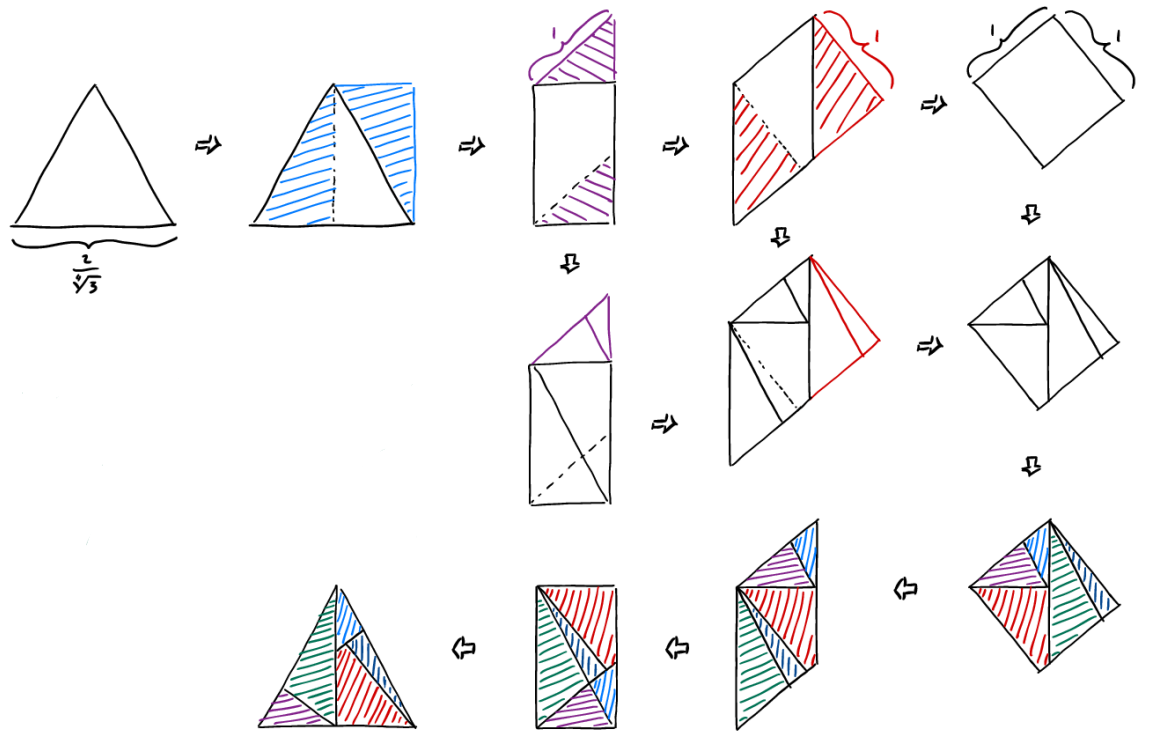
\includegraphics[width = 10cm]{immagini/Dehn_1.png}
\end{figure}

\textcolor{MidnightBlue}{Per passare da un poligono ad un quadrato equivalente [= con la stessa area], è sufficiente spezzarlo in triangoli, poi trasformare i triangoli in rettangoli, poi, passando per un parallelogramma, si trasforma un rettangolo in un altro con uno dei due lati arbitrario.
Infine, portando tutti i rettangoli ad avere un lato uguale, unendoli, e trasformando il nuovo rettangolo in un quadrato, di nuovo col trucco del parallelogramma, si ottiene appunto il quadrato desiderato.}

\begin{note}[L'area secondo Euclide]
	Curiosamente, \href{https://en.wikipedia.org/wiki/Euclid}{\textcolor{purple}{Euclide}} non definisce l'area, ma, dal momento che ci ragiona aggiungendo e togliendo pezzi congruenti, possiamo adattare, a posteriori, una definizione basata sull'equiscomponibilità alla matematica classica.
	Ancora più curiosamente, i ragionamenti di Euclide richiedono in realtà di definire $\text{Area}(A) = \text{Area}(B)$ se e solo se esistono due poligoni $C$ e $D$, rispettivamente non sovrapposti ad $A$ e $B$, equiscomponibili fra loro, tali che $A \cup C$ e $B \cup D$
	sono equiscomponibili. Per dedurre, che, in realtà, due poligoni con la stessa area sono equiscomponibili serve \href{https://en.wikipedia.org/wiki/Archimedean_property}{\textcolor{purple}{l'assioma di Archimede}} che Euclide non aveva. La sistemazione formale di questi concetti è dovuta 
	a \href{https://en.wikipedia.org/wiki/David_Hilbert}{\textcolor{purple}{Hilbert}}, e al XIX secolo.
\end{note}

Ebbene, tutti questi anacronismi solo per dire che \textcolor{purple}{in tre dimensioni questa definizione (per il volume in questo caso) non funziona}, ovvero non è detto che due poliedri con lo stesso volume si possano scomporre in parti congruenti (e quindi non possiamo ottenere l'uno dall'altro come nel caso bidimensionale).

\begin{theorem}[\href{https://en.wikipedia.org/wiki/Max_Dehn}{\textcolor{purple}{Dehn}}]
	Un cubo ed un tetraedro regolare, sia pure aventi il medesimo volume, non si possono scomporre in un numero finito di poliedri congruenti (cioè non sono equiscomponibili).\footnote{Questa proposizione
	e annessa dimostrazione sono un caso particolare della soluzione generale di Dehn al \href{https://en.wikipedia.org/wiki/Hilbert\%27s_third_problem}{\textcolor{purple}{terzo problema di Hilbert}}.}
\end{theorem}

\hspace{-0.43cm}\emph{Dimostrazione.} Supponiamo di avere una funzione $f : \RR \to \RR$ additiva tale che $f(x) = 0$ se e solo se $x$ è un multiplo razionale di $\pi$ - $x = k\pi$ con $k \in \QQ$.\\
	Definiamo il \vocab{valore} di un poliedro come la somma dei valori dei suoi spigoli, definiti, a loro volta, dicendo che il valore di uno spigolo di lunghezza $\ell$ che formi un angolo diedro di ampiezza $\alpha$ e $\ell \cdot f(\alpha)$.\\
	\begin{wrapfigure}[13]{r}{0.2\textwidth}
		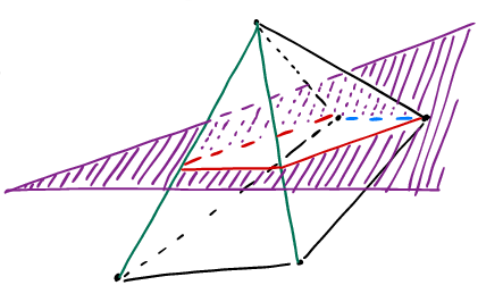
\includegraphics[width=0.17\textwidth]{immagini/cubo_tetraedro.png}
		\hspace{-0.2cm} 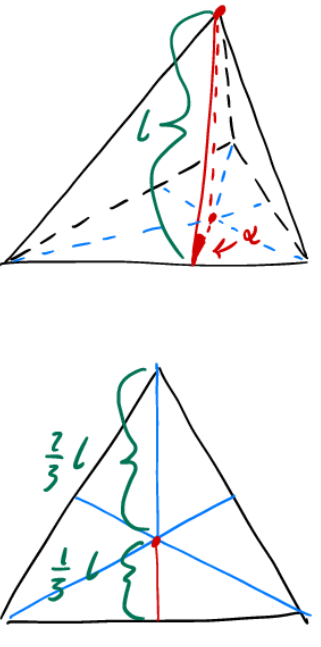
\includegraphics[width=0.13\textwidth]{immagini/angolo_diedro.png}
	\end{wrapfigure}
	Quando tagliamo un poliedro $A$ con un piano, ottenendo così due nuovi poliedri $B$ e $C$, la somma dei valori di $B$ e $C$ equivale al valore di $A$. Infatti, il taglio dà luogo ad alcuni spigoli nuovi, in \textcolor{red}{rosso}, ma la somma dei due angoli 
	diedri, poniamo $\alpha_1$ e $\alpha_2$, che insistono su uno qualunque di essi è $\pi$ e quindi vale che $\ell \cdot f(\alpha_1) + \ell \cdot f(\alpha_2) = \ell \cdot f(\alpha_1 + \alpha_2) = \ell \cdot f(\pi) \overset{\text{def. di $f$}}{=} 0$.\\
	Può dividere spigoli vecchi, in \textcolor{LimeGreen}{verde}, in due,
	poniamo di lunghezza $\ell_1$ e $\ell_2$, senza alterare l'angolo diedro, per cui $(\ell_1 + \ell_2) \cdot f(\alpha) = \ell_1 \cdot f(\alpha) + \ell_2 \cdot f(\alpha)$. Infine, in \textcolor{cyan}{azzurro}, può spezzare l'angolo diedro lasciando inalterata la lunghezza, e si conclude similmente.\\
	Abbiamo concluso quindi che il \vocab{valore} è invariante per equiscomposizioni, pertanto \textcolor{purple}{due figure equiscomponibili devono avere necessariamente lo stesso valore}, non ci resta che costruire $f$. Fissiamo una base $B$ di $\RR$ come spazio vettoriale su $\QQ$ tale che $\pi \in B$
	- ossia estendendo l'insieme linearmente indipendente $\{\pi\}$ (che è una applicazione diretta della proposizione dimostrata in precedenza).
	Definiamo:
	\[ f(\pi q_0 + b_1 q_1 + \ldots + b_n q_n) = b_1 q_1 + \ldots + b_nq_n
		\]
	per ogni $q_0,\ldots,q_n \in \QQ$ e $b_1,\ldots,b_n \in B \setminus \{\pi\}$ \textcolor{MidnightBlue}{- $f$ è quindi la proiezione su un completamento del sottospazio $\pi \QQ$ -}. L'additività di $f$ è conseguenza immediata della $\QQ$-linearità.
	Inoltre, per definizione, $f(x) = 0$ se e solo se $x = \pi q_0$, con $q_0 \in \QQ$.\\
	Ora è chiaro che il valore di un cubo è nullo, perché tutti i diedri hanno ampiezza $\frac{\pi}{2}$, quindi i valori dei singoli spigoli sono tutti nulli e così la loro somma (che per definizione è appunto il valore del cubo).\\
	Vediamo ora che il valore di un tetraedro regolare non è mai nullo - anche se il tetraedro avesse lo stesso volume del cubo -, in tal modo, per quanto detto sul valore, cubo e tetraedro non sono equiscomponibili.\\
	Si vede che gli angoli diedri del tetraedro valgono $\alpha = \arccos\frac 13$, quindi basta dire che questo $\alpha$ non è multiplo razionale di $\pi$, in tal modo il valore de tetraedro sarà non nullo. In altri termini,
	vogliamo verificare che, $n\alpha$, per $n \in \omega$, non è un multiplo intero di $\pi$.\\
	Questo fatto si può esprimere, altresì, dicendo che $z^n \not\in \RR$, dove $z = \cos \alpha + i \sin \alpha \in \CC$ - $z^n = \cos(n\alpha) + i \sin(n\alpha)$, dunque se $n\alpha$ fosse multiplo di $\pi$ si avrebbe $\Im(z^n) = 0 \implies z^n \in \RR$.
	Ora, avendo $\alpha = \arccos \frac 13$, $z = \frac{1}{3}(1 + 2i \sqrt 2)$, e, si vede immediatamente per induzione, che
	$(1 + 2i\sqrt 2)^n = x_n + y_n i \sqrt 2$ per qualche $x_n,y_n \in \ZZ$ (ci basta controllare che $y_n \ne 0$ per ogni $n$). Inoltre, sempre per induzione, riducendo $x_n$ e $y_n$ modulo 3, otteniamo che:
	\begin{itemize}
		\item per $n$ dispari $x_n \equiv 1 \pmod 3$ e $y_n \equiv 2 \pmod 3$.
		\item per $n$ pari e diverso da 0 invece $x_n \equiv 2 \pmod 3$ e $y_n \equiv 1 \pmod 3$.
	\end{itemize}
	In nessun caso, in particolare, si ottiene che $y_n \equiv 0 \pmod 3$, quindi non potrà essere mai che $y_n = 0$, pertanto $z^n$ non sarà mai reale e quindi $n\alpha$ mai multiplo razionale di $\pi$. \hfill $\square$
\newpage
\subsection{Insieme di Vitali}

Vediamo ora un'altra applicazione che da luogo ad un risultato negativo: il \vocab{controesempio di Vitali}.

\begin{definition}[Misura $\sigma$-additiva]
	Una \vocab{misura $\sigma$-additiva} su $\ps(\RR)$ è una funzione $\mu : \ps(\RR) \rightarrow \RR_{\geq 0}\cup\{+\infty\}$, tale che $\mu(\emptyset) = 0$ e, se $\{A_i\}_{i \in \omega}$ è 
	una successione di elementi \textcolor{red}{disgiunti} di $\ps(\RR)$ allora:
	\[ \mu\left(\bigcup_{i \in\omega} A_i\right) = \sum_{i = 0}^{+\infty} \mu(A_i)
		\]
\end{definition}

\begin{definition}[Misura invariante per traslazioni]
	Una misura $\mu$ si dice \vocab{invariante per traslazioni} se $\forall x \in \RR$ e $A \in \ps(\RR)$:
	\[ \mu(A) = \mu(\{y \in \RR | \underbrace{y - x \in A}_{\Mydef A + x}\})
		\]
	cioè la misura di un sottoinsieme di $\RR$ è invariante se lo trasliamo.
\end{definition}

\begin{remark}[Monotonia di una misura]
	Si osserva che se $A \subseteq B \subseteq \RR$, allora $\mu(A) \leq \mu(B)$.
\end{remark}

\begin{proof}
	Si vede che $\mu(B) = \mu(A \sqcup (B \setminus A)) \overset{\text{additività}}{=} \mu(A) + \mu(B \setminus A) \geq \mu(A)$.
\end{proof}

\begin{exercise}
	Esibisci una misura $\sigma$-additiva ed invariante per traslazioni su $\ps(\RR)$.
\end{exercise}

\begin{soln}
	La \href{https://en.wikipedia.org/wiki/Lebesgue_measure}{\textcolor{purple}{misura di Lebesgue}} è una misura $\sigma$-additiva ed invariante per traslazioni su $\ps(\RR)$.
\end{soln}

\begin{proposition}[Controesempio di Vitali]
	Non esiste una misura $\sigma$-additiva e invariante per traslazioni, $\mu : \ps(\RR) \to \RR_{\geq 0} \cup \{+\infty\}$, tale che $\mu([0,1[) = 1$.
\end{proposition}

\begin{proof}
	Supponiamo, per assurdo, che esista una tale misura $\mu$. Cerchiamo degli insiemi disgiunti $A_i \subseteq [0,1[$ con $i \in \omega$ tali che per ogni $i,j \in \omega$ $\mu(A_i) = \mu(A_j)$ e 
	$[0,1[\, = \bigcup_{i \in \omega} A_i$ - stiamo quindi cercando di partizionare $[0,1[$ con un numero numerabile di insiemi disgiunti e aventi tutti la stessa misura -. Se riusciamo scrivere una tale partizione otteniamo appunto un assurdo, infatti:
	\begin{itemize}
		\item se $\mu(A_i) = \mu(A_j) = 0$ per ogni $i,j \in \omega$, allora $\mu([0,1[) = \sum_{i \in \omega} \mu(A_i) = \sum_{i \in \omega}0 = 0 \ne 1 \; \textcolor{red}{\lightning}$.
		\item se $\mu(A_i) = \mu(A_j) = k > 0$ per ogni $i,j \in \omega$, allora $\mu([0,1[) = \sum_{i \in \omega} \mu(A_i) = \sum_{i \in \omega}k = k\cdot \sum_{i \in \omega} 1 = +\infty \ne 1 \; \textcolor{red}{\lightning}$.
	\end{itemize}
	Fissiamo $i \mapsto q_i$ un'enumerazione di $\QQ$, e fissiamo \textcolor{purple}{$B$ base di $\RR$} come $\QQ$-spazio vettoriale. Possiamo assumere WLOG che $b_0 = 1 \in B$, infatti, se così non fosse,
	ci basta prendere $b_0 \in B$ e moltiplicare tutti gli elementi di $B$ per $\frac{1}{b_0}$. Definiamo:
	\[ R_i := \{x \in \RR | x = \textcolor{MidnightBlue}{r_0} \cdot \textcolor{purple}{1} + \textcolor{LimeGreen}{q_i} \cdot \textcolor{purple}{b_1} + \textcolor{MidnightBlue}{r_2} \cdot \textcolor{purple}{b_2} + \ldots + \textcolor{MidnightBlue}{r_n} \cdot \textcolor{purple}{b_n},\;\text{con \textcolor{MidnightBlue}{$r_0,r_2,\ldots,r_n \in \QQ$}}\}
		\]
	cioè l'insieme dei reali che scritti in base $B$ hanno come coefficiente di $b_1$ l'$i$-esimo razionale. Definiamo inoltre $A_i := R_i \cap [0,1[$.
	Siccome la successione $(q_i)_{i \in \omega}$ enumera i razionali, l'unione degli $R_i$, al variare di $i \in \omega$, ci dà proprio - tutte le possibili scritture in base $B$ al variare dei coefficienti razionali - $\bigcup_{i \in \omega}R_i = \RR$,
	inoltre gli $R_i$ sono disgiunti per l'unicità della scrittura in base. Abbiamo quindi che la famiglia $\{R_i\}_{i \in \omega}$ è una partizione di $\RR$, e di conseguenza $\{A_i\}_{i \in \omega}$ è una partizione di $[0,1[$.\\
	Dimostriamo infine che $\mu(A_i) = \mu(A_j)$ per ogni $i,j \in \omega$. Siano $\delta :=(q_j - q_i)b_1$ e $k:=\lceil \delta \rceil$. Consideriamo l'insieme $A_i + \delta$, osserviamo in primis che si ha:
	\begin{align*}
		x \in R_i &\iff x \in \Span(B \setminus\{b_1\}) + q_ib_1 \\
				  &\iff x + \delta \in \Span(B \setminus\{b_1\}) + q_jb_1 &&\textcolor{MidnightBlue}{(q_jb_1 = \delta + q_ib_1)} \\
				  &\iff x + \delta \in R_j
	\end{align*}
	per cui possiamo scrivere $A_i+\delta$ come:
	\begin{align*}
		A_i + \delta &= (R_i + \delta) \cap [\delta,\delta + 1[ \\
					 &= R_j \cap [\delta,\delta + 1[ &&\textcolor{MidnightBlue}{(R_i + \delta = R_j)}\\
					 &= \underbrace{R_j \cap [\delta,k[}_{=: X_1} \cup \underbrace{R_j \cap [k,\delta + 1[}_{=: X_2}
	\end{align*}
	e naturalmente $X_1$ ed $X_2$ sono disgiunti. Similmente per $n \in \omega$:
	\begin{align*}
		x \in R_j &\iff x \in \Span(B \setminus\{b_1,1\}) + \QQ + q_jb_1 \\
				  &\iff x + n \in \Span(B \setminus\{b_1,1\}) + \QQ + q_jb_1 &&\textcolor{MidnightBlue}{(\QQ + n = \QQ)} \\
				  &\iff x + n \in R_j
	\end{align*}
	(in altre parole stiamo semplicemente assorbendo il termine in $\QQ$ nel coefficiente di $b_0 = 1$ nella scrittura in base). Possiamo quindi definire:
	\begin{align*}
		&Y_1 := X_1 - k + 1 = R_j \cap [\delta - k + 1, 1[ \\
		&Y_2 := X_2 - k = R_j \cap [0,\delta - k + 1[
	\end{align*}
	dove abbiamo usato che $R_j = R_j - k + 1$ e $R_j = R_j - k$ per l'osservazione vista prima.
	Di conseguenza $Y_1 \cap Y_2 \subseteq [\delta - k + 1, 1[ \, \cap \,[0,\delta - k + 1[ = \emptyset$ e $Y_1 \cup Y_2 = R_j \cap ([\delta - k + 1, 1[ \, \cup [0,\delta - k + 1[) = R_j \cap [0,1[ = A_j$.
	Mettendo tutto assieme segue quindi:
	\[ \mu(A_j) = \mu(Y_1) + \mu(Y_2) \overset{\text{invar. per trasl.}}{=} \mu(X_1) + \mu(X_2) = \mu(A_i + \delta) \overset{\text{invar. per trasl.}}{=} \mu(A_i)
		\]
\end{proof}

\begin{exercise}[Dimostrazione alternativa]
	Una maniera alternativa di dimostrare la proposizione precedente è come segue:
	\begin{itemize}
		\item considerare la relazione di equivalenza su $[0,1[$ data da $x \sim y \overset{\text{def}}{\iff} x - y \in \QQ$.
		\item fissare un $V \subseteq [0,1[$ che contiene un solo per ogni classe di equivalenza \textcolor{MidnightBlue}{- si usa AC}.
		\item dimostrare che $[0,1[ \subseteq S \Mydef \bigcup_{r \in \QQ \cap ]-1,1[} V + r \subseteq [-1,2[$, per cui $1 \leq \mu(S) \leq 3$.
		\item osservare tuttavia che se $\mu(V) = 0$ allora $\mu(S) = 0$ e se $\mu(V) > 0$ allora $\mu(S) = +\infty$.\footnote{Per la soluzione si veda \href{https://it.wikipedia.org/wiki/Insieme_di_Vitali}{\textcolor{purple}{qui}}.}
	\end{itemize}
\end{exercise}


\subsection{\texorpdfstring{\;Il teorema di Cantor-Bendixson}{Il teorema di Cantor-Bendixson}}
Il teorema di Cantor-Bendixson, che permette di dimostrare l'\vocab{ipotesi del continuo} limitatamente ai sottoinsiemi chiusi di $\RR$, non è tecnicamente, un'applicazione di AC.
Tuttavia è un esempio di come le tecniche insiemistiche - segnatamente la ricorsione transfinita - hanno conseguenze in matematica.\\
Come abbiamo osservato all'inizio del corso, quello di indagare la struttura dei sottoinsiemi chiusi di $\RR$ è stato, forse, uno dei problemi che hanno motivato lo sviluppo della teoria di Cantor. In 
questa sezione ne vedremo, in qualche misura la soluzione.

\paragraph*{Promemoria}\mbox{}\\
Se $S \subseteq \RR$ diciamo che $x \in \RR$ è un \vocab{punto di accumulazione} di $S$, se $x \in \ol{(S \setminus \{x\})}$ \textcolor{MidnightBlue}{- ossia (è nella chiusura di $S\setminus\{x\}$) se esiste una successione $(x_i)_{i \in \omega}$ di 
punti di $S \setminus \{x\}$ tale che $\lim_{i \to +\infty} x_i = x$}. Diciamo che $S \subseteq \RR$ è \vocab{perfetto} se $S$ coincide con l'insieme dei suoi punti di accumulazione ($\mathcal{D}(S)$, il \vocab{derivato} di $S$).

\begin{example}[Gli intervalli chiusi sono insiemi perfetti]
	Un intervallo chiuso $[a,b]$ è un esempio di insieme perfetto.
\end{example}

\begin{exercise}
	Esibire un insieme perfetto non vuoto avente \vocab{parte interna} - ossia $\{x \in S | \; \exists \varepsilon > 0 \; ]x -\varepsilon,x+\varepsilon[ \subseteq S\} = \mathring{S}$ - vuota.
\end{exercise}

\begin{soln}
	L'insieme di Cantor rispetta le proprietà richieste, infatti il suo complementare è unione di segmenti aperti, quindi è un aperto e dunque l'insieme di Cantor è un sottoinsieme chiuso dell'intervallo $[0,1]$.
	Inoltre in un qualsiasi intorno di un punto dell'insieme di Cantor ci sono sia punti dell'insieme sia punti del suo complementare, la prima cosa ci dice che tutti i punti sono aderenti, dunque è perfetto, la seconda ci dice che non ha punti interni,
	dunque ha parte interna vuota.
\end{soln}

\begin{proposition}[Sottoinsiemi perfetti di $\lbrack0,1\rbrack$]
	Se $S \subseteq [0,1]$ è perfetto, allora $|S| = 2^{\aleph_0}$
\end{proposition}

Per dimostrare questa proposizione, è comoda l'osservazione seguente.

\begin{remark}[Ogni perfetto di $\lbrack0,1\rbrack$ contiene due perfetti disugiunti]
	Se $S \subseteq [0,1]$ è perfetto e non vuoto allora esistono $S_1$ e $S_2$ sottoinsiemi di $S$ perfetti, non vuoti e disgiunti.
\end{remark}

\begin{proof}
	Un singoletto non è perfetto, quindi un perfetto ha almeno due punti, $x_1,x_2 \in S$, e supponiamo WLOG $x_1 < x_2$. Ora si danno due casi:
	\begin{itemize}
		\item \underline{se $[x_1,x_2] \subseteq S$}: consideriamo $x_3,x_4$ tali che $x_1 < x_2 < x_3 < x_4$ e definiamo $S_1 = S \cap [0,x_3], S_2 = S \cap [x_4,1]$, questi ultimi sono naturalmente disgiunti, non vuoti, chiusi e senza punti isolati
		(se ce ne fosse uno esisterebbe un intorno che lo isola ovvero che non sta nell'intersezione, ed essendo uno dei due intersecandi un intervallo chiuso l'unica possibilità è che l'intorno che isola il punto 
		nell'intersezione non stia nell'intervallo ma stia solo in $S$, tuttavia in tal modo il punto sarebbe isolato in $S$ che è perfetto $\lightning$).
		\item \underline{se esiste $x_3 \in [x_1,x_2]\setminus S$}: definiamo $S_1 = S \cap [0,x_3]$ e $S_2 = S \,\cap\, [x_3,1]$ (in questo caso intersecando con i chiusi otteniamo ancora un chiuso ed $x_3$ comunque non ci sta dentro, per cui vale lo stesso ragionamento di sopra\footnote{Typo Mamino-}).
	\end{itemize}
\end{proof}

Veniamo ora alla dimostrazione della proposizione.

\begin{wrapfigure}[7]{r}{0.16\textwidth}
	\vspace*{-0.8cm}
	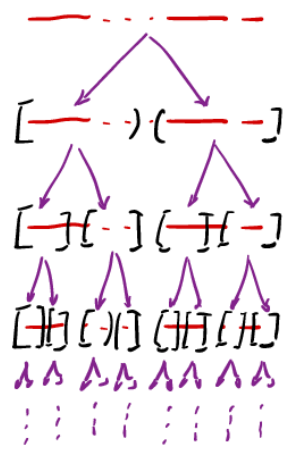
\includegraphics[width=0.15\textwidth]{immagini/perfetti di [0,1].png}
\end{wrapfigure}
\textcolor{MidnightBlue}{L'idea è quella di usare l'osservazione per dividere l'insieme $S$ in due, poi, ricorsivamente ciascuna delle due parti nuovamente in due, e coì via.
Si ottiene un albero binario di sottoinsiemi perfetti di $S$. Quest'albero ha ben $2^{\aleph_0}$ rami infiniti, uno per ogni successione di cifre binarie, e l'intersezione degli insiemi di ogni ramo 
è un'intersezione di compatti uno nell'altro, quindi non vuota. Per cui abbiamo una funzione iniettiva delle successione di cifre binarie a $S$.}

\begin{proof}
	Sia $P$ l'insieme dei sottoinsiemi perfetti di $[0,1]$. Fissiamo $f : P \to P \times P$ che manda $X \in P$ in una coppia $(X_1,X_2)$ con $X_1 \cup X_2 \subseteq X$ e $X_1 \cap X_2 = \emptyset$, e che è ben definita per l'osservazione precedente.\\
	Assegnamo ad ogni sequenza binaria finita, $\sigma : n \to \{0,1\}$, un sottoinsieme perfetto $S_\sigma$ di $S$, procedendo per ricorsione finita su $n$. A questo scopo, data $\sigma : n \to \{0,1\}$ 
	e $b \in \{0,1\}$ indichiamo con $\sigma \frown b$ la sequenza data da $\sigma \cup \{(n,b)\} : n+1 \to \{0,1\}$ - cioè la sequenza $\sigma$ allungata di un passaggio che fa $b$ -. Allora possiamo definire ricorsivamente:
	\[ S_0 = S \qquad S_{\sigma \frown b} = \begin{cases}
		X &\text{se $b = 0$} \\
		Y &\text{se $b = 1$}
	\end{cases}
	\qquad \text{dove $(X,Y) = f(S_\sigma)$}
		\]
	Data una stringa binaria infinita $\tau : \omega \to \{0,1\}$, definiamo infine l'intersezione di tutti i perfetti incontrati man mano che si scende nell'albero:
	\[ S_\tau = \bigcap_{\substack{\sigma = \tau_{|n} \\ n \in \omega}} S_\sigma
		\]
	Osserviamo che, per ogni successione $\tau$, $S_\tau \ne \emptyset$, infatti, per ogni $n \in \omega$, $S_{\tau_{|s(n)}} \subseteq S_{\tau_{|n}}$, poiché ad ogni passaggio aggiungiamo alla successione un perfetto contenuto nel precedente,
	quindi i compatti - siamo in $[0,1]$ quindi sono tutti limitati - non vuoti $S_{\tau_{|n}}$ costituiscono una successione decrescente, per cui - è un fatto topologico - la loro intersezione, che è $S_{\tau}$, è non vuota.\\
	Inoltre se $\tau \ne \rho$ allora $S_\tau \cap S_\rho = \emptyset$ - cioè stringe diverse corrispondono ad intersezioni diverse -, infatti, detto $n$ il minimo indice per cui
	$\tau_{|s(n)} \ne \rho_{|s(n)}$\footnote{Typo Mamino.} - senza perdita di generalità assumiamo $\tau_n = 0$ e $\rho_n = 1$ - abbiamo quindi $S_{\tau_{|s(n)}} = A$ e $S_{\rho_{|s(n)}} = B$ con $A \ne B$ e, per minimalità, $(A,B) = f(S_{\tau_{|n}}) = f(S_{\rho_{|n}})$,
	quindi, per la decrescenza, $S_\tau \subseteq A$ e $S_\rho \subseteq B$ sono disgiunti poiché $A \cap B = \emptyset$.\\
	In conclusione, per ogni $\tau \in 2^\omega$ possiamo scegliere un punto in $S_\tau$ e questa funzione è 
	iniettiva, quindi $2^{\aleph_0} \leq |S|$. D'altro canto $|S| \leq |\RR| = 2^{\aleph_0}$, quindi $|S| = 2^{\aleph_0}$.
\end{proof}

\begin{exercise}
	Dimostrare la proposizione con $\RR$ al posto di $[0,1]$.
\end{exercise}

\begin{exercise}
	In quali passaggi della dimostrazione precedente abbiamo fatto uso dell'assioma della scelta?
\end{exercise}

\begin{exercise}
	Dimostrare la proposizione senza fare uso di AC.
\end{exercise}

\begin{theorem}[Cantor-Bendixson]
	\label{Cantor_Bendixson}
	Sia $C \subseteq \RR$ chiuso. Allora $C = A \cup P$, con $|A| \leq \aleph_0$ e $P$ perfetto.
\end{theorem}

\textcolor{MidnightBlue}{Cioè ogni sottoinsieme chiuso di $\RR$ è unione di un perfetto e di una quantità al più numerabile di punti isolati.}

\begin{proof}
	Dato un sottoinsieme chiuso $C \subseteq \RR$ indichiamo con $X'$ l'insieme dei suoi punti di accumulazione:
	\[ X' = \{a \in \RR | \forall \varepsilon > 0 \; ]a - \varepsilon, a + \varepsilon[ \, \cap \, (X \setminus \{a\}) = \emptyset\}
		\]
	Chiaramente se $X$ è chiuso si ha proprio che i punti di accumulazione sono tutti meno quelli isolati:
	\[ X' = X \setminus \{\text{punti isolati di $X$}\}
		\]
	dove un punto $a \in X$ è isolato se $\exists \varepsilon > 0 \; ]a - \varepsilon, a + \varepsilon[ \, \cap \, X = \{a\}$. Ci servirà l'osservazione seguente: $a \in X$ è un punto isolato di $X$
	se e solo se esiste un intervallo $]s,t[$ aventi estremi razionali che isola $a \in X$, ossia:
	\[ \exists s,t \in \QQ \; s < t \;\land\; ]s,t[ \,\cap\, X  = \{a\}
		\]
	Definiamo ora una successione di sottoinsiemi chiusi a partire da $C$ per ricorsione transfinita come segue:
	\[ C_\alpha := \begin{cases}
		C_0 = C \\
		C_{\alpha + 1} = C_{\alpha}' \\
		C_{\lambda} = \bigcap_{\gamma < \lambda}C_\gamma
	\end{cases}
		\]
	cioè partiamo da $C$ e ad ogni passaggio prendiamo il suo derivato - i suoi punti di accumulazione -, al limite prendiamo semplicemente l'intersezione dei precedenti.
	Per vedere che tutti gli insiemi $C_\alpha$ sono chiusi basta osservare che il derivato di un chiuso è chiuso - di fatto stiamo soltanto togliendo punti isolati - e l'intersezione di chiusi è chiusa.
	Osserviamo inoltre che $\alpha \leq \beta \to C_\beta \subseteq C_\alpha$ - la successione è decrescente -. Definiamo quindi:
	\[ P := \bigcap_{\alpha \in \Ord} C_\alpha = \{a \in \RR | \forall \alpha \in \Ord \; a \in C_\alpha\}\footnote{Non è quindi una vera intersezione, ma un insieme definito per separazione.} \qquad A := C \setminus P
		\]
	Per verificare la tesi dobbiamo quindi dimostrare che $P$ è perfetto e $|A| \leq \aleph_0$.\\
	\textcolor{purple}{$P$ è perfetto}\\
	$P$ è chiuso poiché abbiamo osservato che i $C_\alpha$ sono chiusi e l'intersezione di chiusi è chiusa, occorre quindi dimostrare che $\forall a \in P$, $a$ è un punto di accumulazione per $P$.
	Procediamo per assurdo e consideriamo $a \in P$ isolato, sia $\varepsilon > 0$ tale che $P \,\cap\, ]a - \varepsilon, a + \varepsilon[ = \{a\}$. Per ogni $x \in ]a - \varepsilon, a + \varepsilon[ \setminus\{a\}$ siccome $x \not \in P$,
	esiste $\alpha$ tale che $x \not \in C_\alpha$ - cioè $x$ sta in un intervallo (bucato) che non sta in $P$, per cui non appartiene ad almeno un insieme dell'intersezione -, possiamo quindi prendere $\alpha_x$ minimo per cui $x \not \in C_{\alpha_x}$.
	Sia quindi:
	\[ \beta := \sup_{x \in ]a - \varepsilon, a + \varepsilon[ \setminus\{a\}} \alpha_x
		\]
	\textcolor{MidnightBlue}{cioè il più piccolo ordinale tale per cui $C_\beta$ non contiene alcun elemento di $x \in ]a - \varepsilon, a + \varepsilon[ \setminus\{a\}$}.
	In questo modo l'unico punto dell'intervallo che sta in $C_\beta$ è $a$ - perché per ipotesi sta in $P$, quindi in tutti i $C_\alpha$ -, cioè $C_\beta \,\cap\, ]a - \varepsilon, a + \varepsilon[ = \{a\}$, ma allora $a$ è un punto isolato per $C_\beta$ e quindi per definizione $a \not \in C_{s(\beta)}$, che implica $a \not \in P \;\textcolor{red}{\lightning}$.\\
	\textcolor{purple}{$A$ è al più numerabile}\\
	Per ogni $x \in A$ possiamo considerare $\alpha_x$, il minimo ordinale per cui $x \not \in C_{\alpha_x}$. Osserviamo che $\alpha_x$ deve essere successore,
	perché se fosse limite, avremmo $C_{\alpha_x} = \bigcap_{\gamma < \alpha_x} C_\gamma$, e, non stando nell'intersezione, esisterebbe $\gamma < \alpha_x$ per cui $x \not \in C_\gamma$ che è contro la minimalità di $\alpha_x$.
	Abbiamo quindi che $\alpha_x = s(\beta_x)$, per cui $C_{\beta_x}$ è l'ultimo elemento della successione che abbiamo costruito che contiene $x$.\\
	Siccome $x \in C_{\beta_x}$ e $x \not\in C_{s(\beta_x)} = C'_{\beta_x}$, ciò vuol dire che $x$ è un punto isolato per $C_{\beta_x}$. Per l'osservazione all'inizio possiamo quindi scegliere un intervallo a estremi razionali $]s_x,t_x[$ che isola $x$ in $C_{\beta_x}$.
	A questo punto ci basta definire la funzione:
	\[ A \to \QQ \times \QQ : x \mapsto (s_x,t_x)
		\]
	che è iniettiva. Infatti, siano $x,y \in A$ tali che $]s_x,t_x[ \,=\, ]s_y,t_y[$, supponiamo WLOG che $\beta_x \leq \beta_y$ - cioè $C_{\beta_x} \supseteq C_{\beta_y}$ -, allora:
	\[ y \in\, ]s_y,t_y[ \, \cap \, C_{\beta_y} \subseteq \, ]s_x,t_x[ \, \cap \, C_{\beta_x} = \{x\}
		\]
	dove il contenimento in mezzo vale perché stiamo supponendo gli intervalli uguali e prima abbiamo visto il contenimento dei $C_{\square}$, per cui $x = y$ e quindi abbiamo l'iniettività.
\end{proof}

\begin{corollary}[Vale l'ipotesi del continuo sui chiusi di $\RR$]
	Se $C \subseteq \RR$ è chiuso allora o $|C|=2^{\aleph_0}$ o $|C| \leq \aleph_0$.\footnote{Cioè tra $\aleph_0$ e $2^{\aleph_0}$ non c'è nulla per i chiusi di $\RR$.}
\end{corollary}

\begin{proof}
	Usando il teorema di Cantor-Bendixson scriviamo $C = A \cup P$. Se il perfetto è vuoto, $P = \emptyset$, allora $|C| = |A| \leq \aleph_0$.
	Altrimenti $2^{\aleph_0} = |P| \leq |C| \leq 2^{\aleph_0}$, dove la seconda disuguaglianza è perché $C \subseteq \RR$, mentre la prima uguaglianza 
	deriva dal fatto che abbiamo visto che i perfetti di $\RR$ hanno cardinalità $2^{\aleph_0}$.
\end{proof}

L'esempio seguente mostra come l'ipotesi che $C$ sia chiuso non possa essere omessa.

\begin{example}
	Esiste $S \subseteq \RR$ non numerabile che non contiene alcun insieme perfetto non vuoto.
\end{example}

\begin{proof}
	Sia $|\RR| = 2^{\aleph_0} = \aleph_\alpha$, e sia $f : \ps(\RR) \setminus\{\emptyset\} \to \RR$ una funzione di scelta per i sottoinsiemi di $\RR$. È evidente che:
	\[ 2^{\aleph_0} = |\{\text{intervalli chiusi}\}| \leq |\{\text{perfetti non vuoti}\}| \leq |\{\text{chiusi di $\RR$}\}| = 2^{\aleph_0}
		\]
	quindi esiste una funzione surgettiva - in realtà bigettiva - data da:
	\[ \omega_\alpha \twoheadrightarrow \{\text{perfetti non vuoti}\} : \beta \mapsto P_\beta
		\]
	Definiamo quindi:
	\[ g : \omega_\alpha \to \RR \times \RR : \beta \mapsto (g_1(\beta),g_2(\beta))
		\]
	dove $g_1$ e $g_2$ sono definite per ricorsione transfinita come segue:
	\begin{align*}
		&g_1(\beta) = f(P_\beta \setminus(g_1[\beta] \cup g_2[\beta])) \\
		&g_2(\beta) = f(\RR \setminus (g_1[\beta] \cup g_2[\beta] \cup \{g_1(\beta)\}))
	\end{align*}
	\textcolor{MidnightBlue}{Per cui $g_1$ prende un punto in $P_\beta$ che non sia già stato scelto in precedenza e $g_2$ prende un punto a caso tra quelli non scelti prima compreso $g_1(\beta)$.}\\
	La funzione $g$ è ben definita perché, per ogni $\beta < \omega_\alpha$, si ha $|\beta| < \aleph_\alpha$, quindi $|g_1[\beta]| \leq |\beta| < \aleph_\alpha$ e $|g_2[\beta]|\leq |\beta| < \aleph_\alpha$,
	d'altro canto - per quanto abbiamo visto in generale sui perfetti - $|P_\beta| = 2^{\aleph_0} = \aleph_\alpha$. Di conseguenza, per differenza di cardinalità, $f$ è sempre applicata ad insiemi non vuoti.\\
	Dimostriamo che $S := g_2[\omega_\alpha]$ soddisfa la tesi. In primis osserviamo che non è numerabile, infatti $g_2 : \omega_\alpha \to \RR$ è iniettiva perché, se WLOG $\gamma < \beta$, $g_2(\gamma) \in g_2[\beta]$ - ovvero il punto $g_2(\gamma)$ è nell'elenco di quelli già scelti quindi in $g_2[\beta]$ -
	e $g_2(\beta) = f(\RR \setminus (\ldots g_2[\beta] \ldots)) \ne g_2(\gamma)$ - cioè abbiamo scelto su un insieme dove non c'è $g_2(\gamma)$ -.
	Pertanto si ha $|g_2[\omega_\alpha]| = 2^{\aleph_0}$.\\
	Fissiamo ora un perfetto non vuoto $P_\beta$. Dobbiamo dimostrare che $P_\beta \not\subseteq g_2[\omega_\alpha]$. Ci basta dire che non c'è un suo punto, quindi ci basta mostrare che $g_1(\beta) \not \in g_2[\omega_\alpha]$.
	Supponiamo per assurdo $g_1(\beta) = g_2(\gamma)$ per qualche $\gamma \in \omega_\alpha$. Se $\gamma < \beta$ allora per le definizioni date:
	\[  g_1[\beta] \cup g_2[\beta] \not\ni g_1(\beta) = g_2(\gamma) \in g_1[\beta] \cup \,\textcolor{purple}{g_2[\beta]}\, \;\textcolor{red}{\lightning}
		\]
	Se $\beta \leq \gamma$:
	\[ g_1[\gamma] \cup g_2[\gamma] \cup \{g_1(\gamma)\} \not\ni g_2(\gamma) = g_1(\beta) \in \,\textcolor{purple}{g_1[\gamma]}\, \cup g_2[\gamma] \cup \{g_1(\gamma)\} \;\textcolor{red}{\lightning}
		\]
	quindi $g_1(\beta)$ non è immagine di qualche $\gamma \in \omega_\alpha$ per mezzo di $g_2$.
\end{proof}


\subsection{\texorpdfstring{\;Riepilogo forme equivalenti di AC}{Riepilogo forme equivalenti di AC}}
Abbiamo visto che diverse proposizioni sono equivalenti all'assioma della scelta. Per esempio, fissati gli altri assiomi, AC e 
l'affermazione che ogni insieme è bene ordinabile si implicano vicendevolmente. Elenchiamo le principali forme equivalenti dell'assioma della scelta.

\begin{proposition}[Forme equivalenti dell'assioma della scelta]
	Assumendo gli assiomi di: \hyperref[ax2]{estensionalità}, \hyperref[ax1]{insieme vuoto}, \hyperref[ax3]{separazione}, \hyperref[ax4]{paio}, \hyperref[ax5]{unione},
	\hyperref[ax6]{parti}, \hyperref[ax7]{infinito} e \hyperref[ax8]{rimpiazzamento} le seguenti proposizioni sono equivalenti:
	\begin{itemize}
		\item l'assioma della scelta
		\item ogni funzione surgettiva ha inversa destra
		\item il teorema del buon ordinamento
		\item il lemma di Zorn
		\item ogni cardinalità infinita è un aleph
		\item $\forall X,Y \; |X| \leq |Y| \lor |Y| \leq |X|$
		\item $\forall X \; |X| \leq |\aleph_0| \rightarrow |X \times X| = |X|$.
	\end{itemize}
\end{proposition}

\subsection{\texorpdfstring{\;$|X| = |X \times X| \rightarrow$ AC (Tarski)}{Teorema di Tarski sulla scelta}}
Della proposizione precedente ci rimane da dimostrare solo che per ogni insieme infinito $|X \times X| = |X|$ implica scelta.

\begin{theorem}[Teorema di Tarsk]
	Se per ogni $X$ infinito vale che $|X \times X| = |X|$, allora vale AC.
\end{theorem}

\begin{proof}
	Dato un $X$ infinito cerchiamo un buon ordinamento di $X$. È sufficiente costruire una funzione $g$ che immerge $X$ negli ordinali.\\
	Applicando l'ipotesi a $X \sqcup H(X)$ si ottiene:
	\[ |X \times H(X)| \leq |(X \sqcup H(X)) \times (X \sqcup H(X))| \overset{\text{Hp.}}{=} |X \sqcup H(X)|
		\]
	dove la prima disuguaglianza è una facile immersione\footnote{Ad esempio la mappa $(x,y) \mapsto ((x,0),(y,1))$ è iniettiva.}. Quindi esiste una funzione iniettiva $f : X \times H(X) \hookrightarrow X \sqcup H(X)$. Per ogni $a \in X$ consideriamo la funzione:
	\[ f_a : H(X) \rightarrow X \sqcup H(X) : b \mapsto f(a,b) \, \footnote{Moralmente $f_a = f(a,\cdot)$.}
		\]
	Se l'immagine $f_a[H(X)]$ di $f_a$ fosse contenuta in $X$ (cioè se gli elementi dell'immagine fossero tutte coppie con 0 alla seconda componente), allora avremmo una funzione iniettiva da $H(X)$ ad $X$, che è assurdo per la definizione di numero di Hartogs. Quindi accade necessariamente
	che $f_a[H(X)] \cap H(X) \ne \emptyset$. Definiamo:
	\[ g : X \rightarrow H(X) : a \mapsto \min(f_a[H(X)] \cap H(X))
		\]
	questa funzione è ben definita perché $f_a[H(X)] \cap H(X) \subseteq H(X)$, dunque è un insieme di ordinali, per il quale sappiamo esiste sempre il minimo. Inoltre $g$ è iniettiva perché, se $a \ne b$, allora $g(a) = f(a,\text{qualcosa})$ [per come è definita $f$], e per l'iniettività 
	di $f$, $f(a,\text{qualcosa}) \ne f(b,\text{qualcosa}) = g(b)$. Dunque $g$ è l'immersione cercata di $X$ negli ordinali, pertanto $X$ è bene ordinato, dunque segue il teorema del buon ordinamento e quindi l'assioma scelta.
\end{proof}